\documentclass[12pt]{article}

% packages
\usepackage{amsmath, amssymb}
\usepackage{amsthm}
\usepackage{newtxtext, newtxmath}
\usepackage{geometry}
\usepackage{caption, subfigure}
\usepackage{placeins}
\usepackage{float}
\usepackage{longtable}
\setlength{\LTcapwidth}{\textwidth}
\usepackage{comment}
\usepackage{natbib}
\usepackage{tikz}
\usetikzlibrary{shapes.geometric, arrows.meta, positioning, shadows, calc, fit, backgrounds}
\usepackage[hidelinks]{hyperref}
\usepackage{pdfpages}
\bibliographystyle{abbrvnat}
\setcitestyle{authoryear}

% page settings
\geometry{a4paper}

% theorem styles
\theoremstyle{plain}    % bold title + italics content
\newtheorem{theorem}{Theorem}
\newtheorem{lemma}[theorem]{Lemma}
\newtheorem{proposition}[theorem]{Proposition}

\theoremstyle{definition} % bold title + normal content
\newtheorem{definition}[theorem]{Definition}

\theoremstyle{remark}     %bold title + normal content
\newtheorem{remark}[theorem]{Remark}

\title{Investment Demand Shock and Business Cycle}
\author{Li Xuanguang}
\date{\today}

\begin{document}

% Front cover (first page). cover.pdf is produced separately with XeLaTeX
% (xelatex cover.tex) because it contains the Japanese title. If it has not
% been built yet, fall back to the plain title so main.tex still compiles.
\IfFileExists{cover.pdf}{
\includepdf[pages=-]{cover.pdf}}{\maketitle}

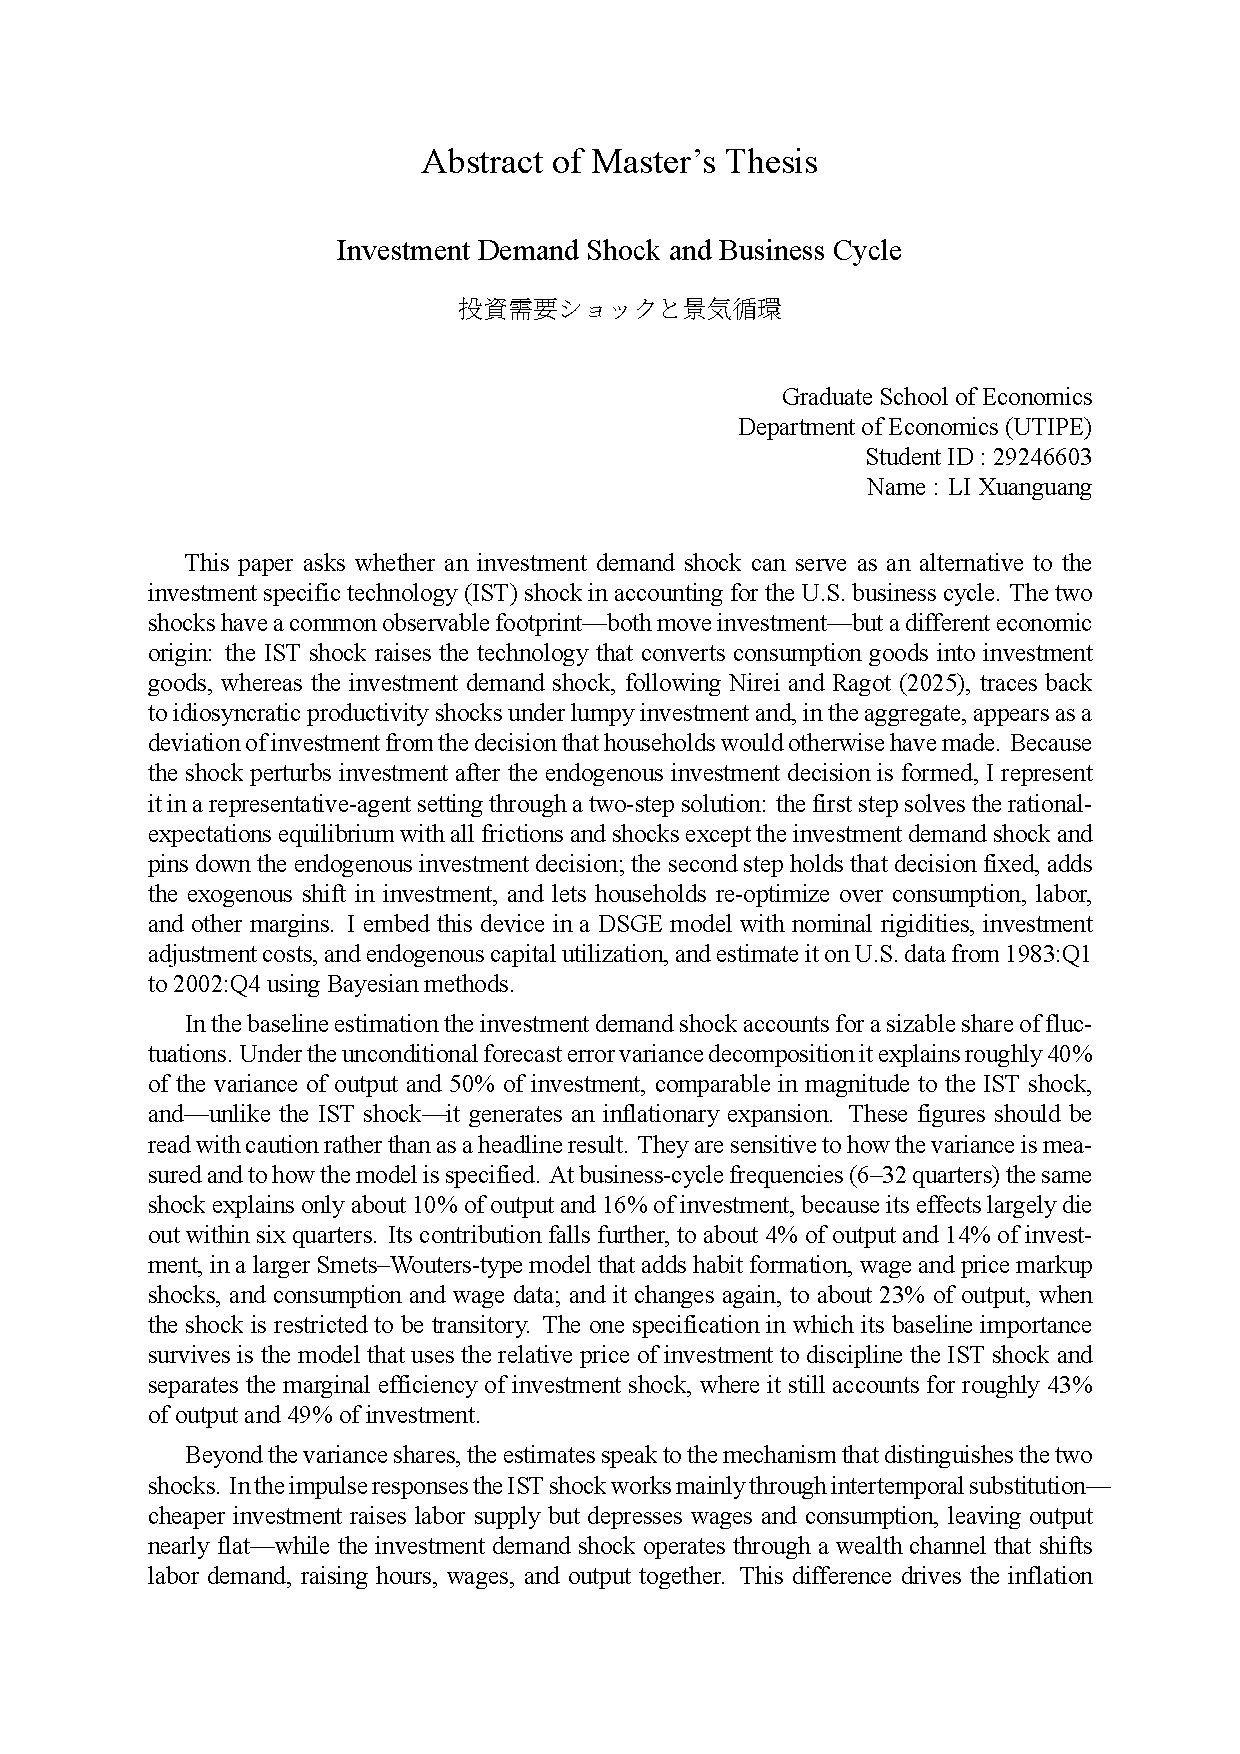
\includepdf[pages=-]{abstract_cover.pdf}

\newpage

\section{Introduction}
\label{sec:introduction}
Investment has been seen as an important part of explaining the business cycle for a long time. It remains the most volatile variable in the macroeconomy. Over the past few decades, the role of investment in the business cycle has been continuously discussed, with new model environments being proposed \citep{greenwoodInvestmentCapacityUtilization1988,greenwoodLongRunImplicationsInvestmentSpecific1997a,fisherDynamicEffectsNeutral2006,justinianoInvestmentShocksBusiness2010,winberryLumpyInvestmentBusiness2021}.

Early research has drawn attention to the investment shock because of the obvious trend in the data on the relative price between investment goods and consumption goods, which implies another trend term in the investment specific technology besides the neutral technology \citep{greenwoodInvestmentCapacityUtilization1988}. After that, quantitative results have been established by \cite{greenwoodLongRunImplicationsInvestmentSpecific1997a} using a calibrated DSGE model, and by \cite{fisherDynamicEffectsNeutral2006} using a structural VAR model. Both of them claimed that the investment shock accounts for about half of the forecast error of the output and the working hours.

A new wave of research about the investment shock is stimulated by \cite{smetsShocksFrictionsUS2007}, who estimated a more frictional model based on \cite{christianoNominalRigiditiesDynamic2005} using Bayesian estimation. Using the same approach, \cite{justinianoInvestmentShocksBusiness2010, justinianoInvestmentShocksRelative2011} argued again that the investment shocks are the main source of the business cycle. While the investment shock shows strong effects on the macroeconomic variables, there are other candidates being proposed to account for the business cycle. \cite{christianoRiskShocks2014} and \cite{kamberFinancialFrictionsRole2015} argued that investment shock is less important once the model includes financial friction and shocks in the financial market.

Though I use the name of investment shock in the previous paragraphs, there are various kinds of specification being discussed. Among them, the most classic one is the investment specific technology (IST) shock, which increases the technology level to produce the investment goods by the consumption goods \citep{greenwoodLongRunImplicationsInvestmentSpecific1997a, fisherDynamicEffectsNeutral2006, justinianoInvestmentShocksBusiness2010}. Besides, \cite{justinianoInvestmentShocksRelative2011, kamberFinancialFrictionsRole2015} distinguished the IST shock from the marginal efficiency of investment (MEI) shock, which represents the technology level to produce the capital goods by the investment goods. However, the difference between these two shocks rely on the detailed modeling of the capital production process. If the capital production is modelled by one capital law of motion equation, then those two shocks cannot be distinguished in their effect, and thus I make no clarification between them except for Section~\ref{sec:robustness:mei}. In addition, there are many works discussed the IST news shock, in the sense that the shock is known by agents now but will affect the economy several periods after \citep{schmitt-groheWhatsNewsBusiness2012, benzeevInvestmentSpecificNewsShocks2015, liaoNewsShocksInvestmentspecific2023}. However, this kind of shock is beyond the scope of this paper.

Despite the IST shock has been considered as an important driving force of the business cycle, it fails to generate the comovement between the consumption, investment and inflation. To solve the comovement problem, \cite{nireiOriginsPropagationAnimal} proposed an investment demand shock based on a model featuring the firms' heterogeneity and the lumpy investment assumption. By the calibrated model, the investment demand shock generates the comovement between consumption and investment. While the shock is traced back to the idiosyncratic productivity shock, on the aggregate level, in macro level it presents a deviation of investment from the original investment decision made in the shock-free environment. Because of this, the investment demand shock can also be represented in a DSGE model without heterogeneity, and be estimated using the same approach with \cite{smetsShocksFrictionsUS2007}.

However, since this shock requires to fix the endogenous investment decision, the solution method of the rational expectation equilibrium needs to be separated into two steps. In the first step, the model includes all shocks and frictions except for the investment demand shock, from where the endogenous investment decision is solved. In the second step, the investment is decided by both the endogenous investment decision and the exogenous investment demand shock. It is worth pointing out that the endogenous investment decision cannot be changed in the second step, and thus investment demand is exogenously increased by the shock. Although the investment decision is fixed, households can still adjust their decisions on other terms, such as consumption and labor input, and thus the second step solves another equilibrium. This equilibrium, finally, will be used to compute the likelihood.

The identification strategy is not direct---it is hard to directly identify invesetment demand shock by data, as the shock is originated from idiosyncratic productivity shock. Moreover, though we can use relative price of invesetment goods as the proxy for IST shock in some sense, there is still a concern that we might attribute all residuals to invesetment demand shock. Therefore, I postpone this exercise to a later section and rely on the theoretical difference---whether the comovement between consumption, investment and inflation---to identify two shocks in the baseline result. However, due to the high-dimensional parameter space, the comovement difference is hard to test among all combinations of parameter values. Therefore, I claim the shortage of such identification strategy.

Section~\ref{sec:model} introduces the baseline model. Section~\ref{sec:solution} presents the solution method and incorporates the investment demand shock. Section~\ref{sec:estimation} describes the Bayesian estimation, and Section~\ref{sec:results} reports the benchmark results. Section~\ref{sec:robustness} provides robustness checks, and Section~\ref{sec:conclusion} concludes.

\section{Baseline Model}\label{sec:model}
    The baseline model is based on \cite{herbstBayesianEstimationDSGE2015} and \cite{smetsShocksFrictionsUS2007}. I selected some model settings to maintain the fit to the data, including price and wage rigidity, investment adjustment cost, and endogenous capital utilization ratio. However, some settings are left out in the baseline model to keep the solution clean, such as habit formation and price indexation.

    I first specify the model without the investment demand shock, and then add the shock in Section~\ref{sec:solution}.

    \subsection{Household}
    There is a continuum of households indexed on $[0,1]$. For simplicity of notation, the index of the household is omitted in the following equations. The representative household owns the firms and solves the dynamic optimal problem over consumption $c_t$, hours worked $\ell_t$, nominal bonds $B_t$, investment $i_t$, capital $k_t$, and capital utilization $u_t$.
        \begin{equation}
            \max\limits_{c, b, i, k, l, u} \,\mathbb{E}_t \sum_{k=0}^{\infty} \beta^k \left(\frac{(c_{t+k} / \gamma^{t+k})^{1-\sigma} - 1}{1 - \sigma} - \chi\frac{\ell_{t+k}^{\sigma_\ell + 1}(j)}{\sigma_\ell + 1}\right)
        \end{equation}
    
    In the objective function, $\gamma$ is the growth rate of the labor-augmented technology, which is used to generate a trend in the state variables. Usually, if we use detrended data, there is no need to add this term. However, the process of detrending itself includes some operations on the data, which are not explained in the model. To maintain the integrity of the estimation process, I use $\gamma$ to fit the non-detrended data.

    Following \cite{herbstBayesianEstimationDSGE2015}, I assume the representative household derives utility from effective consumption, defined as absolute consumption scaled by the trend in labor-augmenting technology. This formulation mathematically guarantees the existence of a balanced growth path and the convenience of representing the marginal utility, as we can directly define the detrended consumption $\tilde{c}_{t+k} = c_{t+k} / \gamma^{t+k}$ within it.
    
    The budget constraint appears in the following equation:
    \begin{equation}
        c_t + i_t + \frac{b_{t+1}}{R_{t+1}P_t} = r^k_t k_{t-1}u_t - a(u_t)k_{t-1} + \frac{b_t}{P_t} + w_t \ell_t - \frac{\tau_t}{P_t} + \frac{d_t}{P_t}.
    \end{equation}
    where $b_t$ and $R_t$ denote nominal bonds and the nominal interest rate. $\tau_t$ is the nominal tax, and $d_t$ is the nominal dividend from the firms they own. $a(u_t)k_{t-1}$ is the adjustment cost of capital utilization. $a(\cdot)$ is a function defined on $[0, 1]$, satisfying $a(1)=0$ and $a''(1) > 0$. Endogenous capital utilization allows capital to be adjusted when facing shocks, even though capital is still a predetermined variable, and the adjustment cost of capital utilization smooths the adjustment process.

    The law of motion of capital adds several additional terms compared with the standard one.
    \begin{equation}
        k_{t+1} = (1 - \delta) k_t + \mu_{s, t}\left[1 - S\left(\frac{i_t}{i_{t-1}}\right)\right] i_t
    \end{equation}

    The first one is the investment specific technology shock $\mu_{s, t}$, which can be assumed to follow a stationary AR(1) process without incorporating the relative price of investment.
    \begin{equation}
        \ln \mu_{s, t} = (1 - \rho_{i}) \ln \mu_{s} + \rho_{s}\ln \mu_{s, t-1} + \varepsilon_{s, t}, \,\, \varepsilon_{s, t} \sim \text{i.i.d. } \mathcal{N}(0, \sigma_s^2)
    \end{equation}

    The second one is the investment adjustment cost $S\left(\frac{i_t}{i_{t-1}}\right)$. I use the function form $S(x) = \frac{\phi_i}{2}(x - \gamma)^2$, indicating that if the growth of the investment is above or below the balanced path growth rate, then an additional adjustment cost should be charged. The setting is important because the investment would otherwise be very sensitive to the shocks, which fails to match the comovement in the data \citep{winberryLumpyInvestmentBusiness2021} and causes unrealistic impulse response functions.

    From the household's optimal problem, we obtain the following first-order conditions. Let $Q_t$ denote the ratio of the Lagrange multiplier on the law of motion of capital to the Lagrange multiplier on the budget constraint, which captures the relative marginal utility between consumption and investment. $Q_t$ has the following relation to Tobin's $Q$: $\text{Tobin's }Q = Q_t \mu_{s, t}$. Define gross inflation as $\pi_{t+1}\equiv P_{t+1}/P_t$.
    \begin{align}
        &\Lambda_{t,t+1} \equiv \frac{\beta}{\gamma}\left(\frac{c_{t+1}/\gamma^{t+1}}{c_t/\gamma^t}\right)^{-\sigma}
        \label{eq:sdf}\\
        &\begin{aligned}
        \label{eq:inv_foc}
        1 &= Q_t\,\mu_{s,t}\left(1 - S\left(\frac{i_t}{i_{t-1}}\right) - S'\left(\frac{i_t}{i_{t-1}}\right)\frac{i_t}{i_{t-1}}\right)
        \\
        &\qquad+ \mathbb{E}_t\left[\Lambda_{t,t+1}\,Q_{t+1}\,\mu_{s,t+1}\,S'\left(\frac{i_{t+1}}{i_t}\right)\left(\frac{i_{t+1}}{i_t}\right)^2\right],\\
        \end{aligned}\\
        &Q_t = \mathbb{E}_t\left[\Lambda_{t,t+1}\,\big(r_{t+1}^k u_{t+1} - a(u_{t+1}) + (1-\delta)Q_{t+1}\big)\right],
        \label{eq:q_euler}\\
        &1 = \mathbb{E}_t\left[\Lambda_{t,t+1}\,\frac{R_{t+1}}{\pi_{t+1}}\right]
        \label{eq:euler_bond},\\
        &w_t = \chi\,\ell_t^{\sigma_\ell}\,\gamma^t\left(\frac{c_t}{\gamma^t}\right)^{\sigma}, \\
        &r_t^k = a'(u_t)
        \label{eq:util_foc}.
    \end{align}

    \subsection{Final Goods Producer}
    This part of model is standard, where perfectly competitive firms produce the final goods $Y_t$ using a CES aggregator. They solve the optimal problem,
    \begin{equation}
        \begin{aligned}
             \max\limits_{Y_t, y_t(j)}\, & P_t Y_t - \int_{0}^{1} p_t(j)y_t(j)\, dj \\
             \text{s.t.  } & Y_t = \left(\int_{0}^{1} y_{t}(j)^{\nu - 1}\, dj\right)^{\frac{1}{\nu - 1}}.
        \end{aligned}
    \end{equation}
    
    Therefore, from the first-order condition, the demand for each intermediate good follows:
    \begin{equation}
        y_t(j) = \left(\frac{p_t(j)}{P_t}\right)^{-\nu} Y_t,
    \end{equation}
    where $P_t$ follows
    \begin{equation}
        P_t = \left(\int_{0}^{1} p(j)^{\frac{\nu - 1}{\nu}}\, dj\right)^{\frac{\nu}{\nu - 1}}.
    \end{equation}

    Alternatively, we could define the price markup shock by replacing the fixed parameter $\nu$ by a time-varying random variable.

    \subsection{Intermediate Goods Producer}
    Each intermediate goods producer has to solve both the cost minimization problem and the dynamic pricing problem.
    
    The cost minimization problem is
    \begin{equation}
        \min\limits_{k^s_t(j), n_t(j)}\, r_t^k k^s_t(j) + w_t n_t(j)
    \end{equation}
    subject to their production technology,
    \begin{equation}
        y_t(j) = \mu_{a, t} k^s_t(j)^{\alpha}\left(\gamma^t n_t(j)\right)^{1-\alpha},
    \end{equation}
    where $\mu_{a, t}$ is the aggregate productivity technology, following
    \begin{equation}
        \ln \mu_{a, t} = (1 - \rho_a) \ln \mu_{a} + \rho_a \ln \mu_{a, t-1} + \varepsilon_{a, t}, \,\, \varepsilon_{a, t} \sim \text{i.i.d. } \mathcal{N}(0, \sigma_a^2).
    \end{equation}

    $\gamma^t$ ($\gamma>1$) is the labor-augmented technology, which helps derive the balanced growth path. In addition, $K^s_t$ denotes the capital service, which will be influenced by the capital utilization $u_t$ under general equilibrium conditions.

    Cost minimization yields the cost function. However, as the production function has constant returns to scale, the marginal cost is solved as well:
    \begin{equation}
        mc_t(j) = \frac{1}{\alpha^\alpha (1-\alpha)^{1-\alpha} \gamma^{t(1-\alpha)}}\frac{w_t^{1-\alpha} (k_t^s)^{\alpha}}{\mu_{a,t}}.
    \end{equation}

    The Calvo pricing problem is described below.
    \begin{equation}
        \begin{aligned}
        \max\limits_{p_t(j)}\, &\mathbb{E}_t \sum_{k=0}^{\infty} \theta_p^k \Lambda_{t+k, t} \left(p_t(j) y_{t+k}(j) - P_{t+k} mc_{t+k}(j)\right) \\
        \text{s.t.   } & y_{t+k}(j) = \left(\frac{p_t(j)}{P_{t+k}}\right)^{-\nu},
        \end{aligned}
    \end{equation}
    where $\theta_p$ is the Calvo probability of not being allowed to reoptimize one's price, and $\Lambda_{t+k, t}$ is the stochastic discount factor between period $t+k$ and period $t$ defined in equation~\eqref{eq:sdf}.

    I drop the price indexation, which allows firms to move their prices according to the inflation in the last period even though they are not allowed to reoptimize their prices, because \cite{smetsShocksFrictionsUS2007} shows the model has a higher posterior likelihood without this setting.

    \subsection{Wage Setting}
    Instead of modeling a detailed intermediate labor sector, the baseline model uses a simplified wage setting equation to introduce the sticky wage, following \cite{nireiOriginsPropagationAnimal}.
    \begin{equation}
        w_t = \left(\frac{L_t^{\sigma_\ell}}{C_t^{-\sigma}}\right)^{\theta_w} w^{1 - \theta_w}
    \end{equation}
    where $w$ is the steady-state real wage. Similar to the Calvo pricing problem, the equation roughly means that only a $\theta_w \in (0,1)$ part of wage contracts can be reset to match the current marginal rate of substitution between hours worked and consumption. Meanwhile, the rest of the $1 - \theta_w$ part can only keep the steady-state real wage.

    Comparing with the standard sticky wage setting in \cite{erceg2000optimal}, this simplified wage-setting equation assumes a perfectly competitive labor market, and thus there is no wage markup if the firms are allowed to reset the wage contract. In addition, the trapped wage is on the steady-state level, which can be taken as the optimal wage setting before a shock has happened.

    Another property of this equation is that the implied wage markup is not constant. To see this, we can simply calculate 
    
    $$\frac{w_t}{MRS_t} = \left(\frac{L_t^{\sigma_\ell}}{C_t^{-\sigma}}\right)^{ \theta_w - 1} w^{1 - \theta_w} = MRS_t^{\theta_w - 1}w^{1 - \theta_w}.$$

    The wage markup increases a lot when the $MRS_t$ approaches $0$, which means the wage markup can absorb much of the decrease of the $MRS_t$ in this regime and keeps the change of the real wage smooth. This mechanism is shown by \cite{justinianoInvestmentShocksBusiness2010} to be important in accounting for the role of the investment shock in the business cycle.

    \subsection{Government}
    The government performs the monetary and fiscal policy. The central bank follows a standard Taylor rule,
    \begin{equation}
        R_t = \left(\pi^* r \left(\frac{\pi_t}{\pi^*}\right)^{\psi_{\pi}} \left(\frac{Y_t}{Y_t^{n}}\right)^{\psi_y}\right)^{1 - \rho_R} R_{t-1}^{\rho_R}\exp(\varepsilon_{R,t})
    \end{equation}

    $\pi^*$ is the targeted inflation rate of the central bank, and $r$ is the steady-state real interest rate. The nominal interest rate is set according to the deviation of inflation $\pi_t$ from the targeted inflation rate and of output $Y_t$ from the natural output $Y^n_t$. Finally, $R^{\rho_R}_{t-1}$ smooths the change of the nominal interest rate, and $\varepsilon_{R,t}$ is the monetary policy shock, with $\varepsilon_{R,t} \sim \text{i.i.d. } \mathcal{N}(0, \sigma_R^2)$ across time.

    The fiscal policy part includes a government budget constraint and an exogenous government spending process.
    \begin{equation}
            P_t G_t + R_{t-1} B_{t-1} = B_t + T_t
    \end{equation}
    
    Government spending, $G_t$, follows an output stabilization rule and an exogenous government spending process \citep{leeperDynamicsFiscalFinancing2010}.
    \begin{equation}
        G_t = \left(\frac{Y_t}{Y}\right)^{-\phi_g} \mu_{g, t}
    \end{equation}

    $\mu_{g, t}$ follows,
    \begin{equation}
        \ln \mu_{g, t} = (1 - \rho_g) \ln \mu_{g} + \rho_{g}\ln\mu_{g, t-1} + \varepsilon_{g, t}, \,\, \varepsilon_{g, t} \sim \text{i.i.d. } \mathcal{N}(0, \sigma_g^2).
    \end{equation}

    \subsection{Resource Constraint}
    First we define the aggregate variables from the integration of households' optimal choices,
    \begin{equation}
        \begin{aligned}
            &C_t = \int_{0}^{1} c_t(j) \, dj, \,\, 
            I_t = \int_{0}^{1} i_t(j) \, dj, \,\,
            L_t = \int_{0}^{1} \ell_t(j) \, dj,\,\,\\
            &K_t = \int_{0}^{1} k_t(j) \, dj, \,\,
            B_t = \int_{0}^{1} b_t(j)\, dj,
        \end{aligned}
    \end{equation}

    Since capital utilization $u_t$ is only associated with the real interest rate of capital in equation~\eqref{eq:util_foc}, it is the same across all households. After integrating on the variables of $k^s_t(j)$ and $n_t(j)$ on the firms' side, and then applying the equilibrium condition, we can get
    \begin{equation}
        \begin{aligned}
            Y_t &= C_t + I_t + G_t + a(u_t)K_{t-1} \\
            K_t^s &= u_t K_{t-1} \\
            N_t & = L_t
        \end{aligned}
    \end{equation}

    The government bond market clears according to Walras' law.


\section{Equilibrium Solution Method}
\label{sec:solution}
This section introduces the investment demand shock to the model and the solution method. The solution requires multiple parallel models---one for solving the endogenous investment demand, and two for solving the natural output.

\subsection{Investment Demand Shock and Second-stage Model}
The starting point is the investment level decided by the baseline model, which is denoted as $I^*_t$. After the equilibrium is established in the baseline model, the investment demand shock $\varepsilon_{d, t}$ is revealed, causing total investment to increase exogenously. Specifically, $\mu_{d, t}$ is the exogenous investment demand process, following
\begin{equation}
    \ln \mu_{d, t} = (1 - \rho_d) \ln \mu_d + \rho_d \ln \mu_{d, t-1} + \varepsilon_{d, t},\,\, \varepsilon_{d, t} \sim \mathcal{N}(0, \sigma_{d, t}^2)
\end{equation}
and the total investment becomes
\begin{equation}\label{eq:invest_law}
    I_t = \mu_{d, t} I^*_t .
\end{equation}

As all households are representative, the increase in aggregate investment is equivalent to each household increasing its investment $i_t^*$ by $\mu_{d,t}$. Therefore, we can specify the new optimal problem for each household.
\begin{equation}\label{eq:new_hh_optimal}
    \begin{aligned}
        \max\limits_{c, b, k, l, u} \, &\mathbb{E}_t \sum_{k=0}^{\infty} \beta^k \left(\frac{(c_{t+k} / \gamma^{t+k})^{1-\sigma} - 1}{1 - \sigma} - \chi\frac{\ell_{t+k}^{\psi + 1}(j)}{\psi + 1}\right) \\
        \text{s.t.  } & c_t + \mu_{d, t} i^*_t + \frac{b_{t+1}}{R_{t+1}P_t} = r^k_t k_{t-1}u_t - a(u_t)k_{t-1} + \frac{b_t}{P_t} + w_t \ell_t - \frac{\tau_t}{P_t} + \frac{d_t}{P_t} \\
        &k_{t+1} = (1 - \delta) k_t + \mu_{s, t}\left[1 - S\left(\frac{\mu_{d, t} i^*_t}{i_{t-1}}\right)\right] \mu_{d,t} i^*_t
    \end{aligned}
\end{equation}

The difference between this optimal problem and the one in Section~\ref{sec:model} lies in the control variables. Equation \eqref{eq:new_hh_optimal} states that investment is no longer a control variable. Instead, it is decided by the investment law described in equation \eqref{eq:invest_law}, and thus we do not have the first-order condition with respect to investment. This kind of specification is not common, because it actually says households are making the investment decision irrationally---the investment is not decided by the first-order condition. However, \cite{nireiOriginsPropagationAnimal} provides the micro-foundation of such shock, which is generated from firms' idiosyncratic productivity shocks and the complementary movement between firms.

Following the exogenous investment required by the household, the economy should solve the equilibrium again, which will be finally used to calculate the likelihood. The reason why the investment demand shock cannot be compounded with the baseline model is that the household will adjust their investment according to the realization of the shock otherwise. 

\subsection{Frictionless Parallel Models}
To solve the natural output used in the Taylor's rule, two frictionless parallel models should be introduced, one of which corresponds to the baseline model, and the other of which corresponds to the second-stage model. The two frictionless parallel models are nearly the same, except for the setting related to the investment demand shock.

Inside each frictionless parallel model, all nominal variables are excluded, and the wage sticky parameter $\theta_w$ is set to zero so that the real wage equals the marginal rate of substitution between hours worked and consumption.

\begin{figure}[htbp]
    \centering
    \resizebox{0.9\textwidth}{!}{%
    % --- Define standard styles for consistency ---
\tikzset{
    % Basic model box style
    base_model/.style={
        rectangle, 
        minimum width=6.5cm,
        minimum height=3.5cm,
        align=center,
        font=\sffamily\normalsize,
        inner sep=10pt
    },
    % Model title style
    model_title/.style={
        font=\sffamily\bfseries\normalsize,
        yshift=-8pt
    },
    % Model description style
    model_desc/.style={
        font=\sffamily\normalsize,
        color=black,
        align=center,
        text width=6cm,
        yshift=2pt
    },
    % Pre-stage models (Blue theme)
    pre_model_style/.style={
        base_model,
        draw=black,
        top color=white,
        bottom color=white,
    },
    % Post-stage models (Green theme)
    post_model_style/.style={
        base_model,
        draw=black,
        top color=white,
        bottom color=white,
    },
    % Connection arrows for investment
    inv_arrow/.style={
        draw,
        -Latex,
        line width=1.5pt,
        color=black
    },
    % Connection arrows for natural output/Taylor rule
    yn_arrow/.style={
        draw,
        -Latex,
        line width=1.5pt,
        color=black
    },
    % Parallel relationship style
    parallel_link/.style={
        draw,
        Latex-Latex,
        dashed,
        line width=1pt,
        color=black
    },
    % Labels for arrows
    label_node/.style={
        midway,
        fill=white,
        draw=white,
        font=\sffamily\bfseries\small,
        inner sep=3pt,
        opacity=1,
        text opacity=1
    },
    % ERROR / MISTAKE STYLE
    error_arrow/.style={
        draw,
        -Latex,
        line width=1.5pt,
        color=red!70,
        dashed
    },
    error_label/.style={
        midway,
        fill=red!10,
        draw=red!50,
        text=red!70!black,
        font=\sffamily\bfseries\small,
        rounded corners=3pt,
        align=center
    }
}

\begin{tikzpicture}[node distance=3cm and 2.5cm]

% =========================================
% ROW 1: PRE-STAGE MODELS
% =========================================

% Pre Flexible Model
\node (preFlex) [pre_model_style] {};
\node [model_title, anchor=north] at (preFlex.north) {Pre-Flexible Model};
\node [model_desc, anchor=center] at (preFlex.center) {
    Frictionless parallel model.\\
    No investment demand variables.\\
    Solves for natural output ($Y^n$).
};

% Pre Model
\node (pre) [pre_model_style, right=of preFlex] {};
\node [model_title, anchor=north] at (pre.north) {Pre Model};
\node [model_desc, anchor=center] at (pre.center) {
    Sticky price model.\\
    No investment demand variables.\\
    Uses $Y^n$ in the Taylor rule.
};


% =========================================
% ROW 2: POST-STAGE MODELS
% =========================================

% Post Flexible Model
\node (postFlex) [post_model_style, below=of preFlex] {};
\node [model_title, anchor=north] at (postFlex.north) {Post-Flexible Model};
\node [model_desc, anchor=center] at (postFlex.center) {
    Frictionless parallel model.\\
    Investment is fixed.\\
    Solves for post-stage $Y^n$.
};

% Post Model
\node (post) [post_model_style, right=of postFlex] {};
\node [model_title, anchor=north] at (post.north) {Post Model};
\node [model_desc, anchor=center] at (post.center) {
    Sticky price model.\\
    Contains investment demand.\\
    Investment is fixed (from Pre Model).
};


% =========================================
% CONNECTIONS
% =========================================

% Investment Connections (Vertical)
\draw [inv_arrow] (preFlex.south) -- (postFlex.north)
    node [label_node] {$I^*$};

\draw [inv_arrow] (pre.south) -- (post.north)
    node [label_node] {$I^*$};

% Natural Output Connections (Horizontal)
\draw [yn_arrow] (preFlex.east) -- (pre.west)
    node [label_node] {$Y^n$};

\draw [yn_arrow] (postFlex.east) -- (post.west)
    node [label_node] {$Y^n$};


% =========================================
% ANNOTATIONS
% =========================================
\begin{pgfonlayer}{background}
    % Track Backgrounds
    \node [fit=(preFlex)(postFlex), rounded corners=15pt, inner sep=15pt, label={[font=\sffamily\bfseries\normalsize, color=black]above:Frictionless Track}] (flexTrack) {};
    \node [fit=(pre)(post), rounded corners=15pt, inner sep=15pt, label={[font=\sffamily\bfseries\normalsize, color=black]above:Sticky Track}] (stickyTrack) {};
    
    % Stage Backgrounds (invisible but used for labels)
    \node [left=1.5cm of preFlex, font=\sffamily\bfseries\normalsize, anchor=south, color=black] {Pre-stage};
    \node [left=1.5cm of postFlex, font=\sffamily\bfseries\normalsize, anchor=south, color=black] {Post-stage};
\end{pgfonlayer}

\end{tikzpicture}

    }
    \caption{Link between the baseline model, the second-stage model with investment demand shock, and the frictionless parallel models used to compute endogenous investment and natural output.}
    \label{fig:parallel_model}
\end{figure}

The relations between all models are illustrated in Figure~\ref{fig:parallel_model}. Basically, starting from the frictionless baseline model, we solve the endogenous investment and natural output. The endogenous investment is then sent to the frictionless second-stage model, and the natural output to the sticky baseline model. Next, another endogenous investment is solved from the sticky baseline model and another natural output from the frictionless second-stage model. Finally, combining the new endogenous investment and natural output, I solve the second-stage model.

\subsection{Detrending and Log-linearization}
As the model is endowed with a growth trend, the detrended state variables should be defined before solving the steady state. Specifically, define
\begin{equation}
    \tilde{Y}_t = \frac{Y_t}{\gamma^t},\,\,
    \tilde{C}_t = \frac{C_t}{\gamma^t},\,\,
    \tilde{I}_t = \frac{I_t}{\gamma^t},\,\,
    \tilde{K}_t = \frac{K_t}{\gamma^t},\,\,
    \tilde{K}^s_t = \frac{K_t^s}{\gamma^t},\,\,
    \tilde{w}_t = \frac{w_t}{\gamma^t}
\end{equation}

After rewriting the first-order conditions in terms of the detrended model, we can solve the steady state and the log-linearized model. The detailed derivation is put in Appendix~\ref{app:model}. 

\section{Estimation}
\label{sec:estimation}
This section describes the estimation method, including data selection, priors and posteriors of parameters. The methodology follows \cite{smetsShocksFrictionsUS2007} and \cite{justinianoInvestmentShocksBusiness2010}.

\subsection{Data}
The data set contains U.S. data on GDP growth rate, inflation rate, the federal funds rate, hours worked, investment growth rate, and government spending growth rate. The data period is from 1983:Q1 to 2002:Q4. The period selection is based on three considerations. First, since the economic model assumes a constant linear growth trend, we may face the problem of changing growth rates if we use a data set over long periods. Second, the data is selected to be comparable with \cite{justinianoInvestmentShocksBusiness2010}, who used the data from 1954:Q3 to 2004:Q4. Third, the data period avoids the periods where the economy faced the zero-lower bound constraint, as the model lacks a clear picture of monetary policy in such regimes.

All data are collected from the FRED database, and are processed to represent per-capita levels because there is no detailed modeling of population growth in the baseline model. The detail of the data process is described in Appendix~\ref{app:data}.
\begin{equation}\label{eq:observation}
    \begin{bmatrix}
        \Delta \ln GDP_t \\
        \Delta \ln P_t \\
        FEDFUNDS_t\\
        \ln HOURS_t \\
        \Delta \ln INV_t \\
        \Delta \ln GOV_t \\
    \end{bmatrix}
    =
    \begin{bmatrix}
        100 \ln \gamma \\
        400\pi_{ss} \\
        400R_{ss} \\
        \bar{\ell}\\
        400\ln \gamma \\
        400\ln \gamma \\
    \end{bmatrix}
    +
    \begin{bmatrix}
        \hat{y}_t - \hat{y}_{t-1} \\
        \hat{\pi}_t \\
        \hat{R}_t \\
        \hat{\ell}_t\\
        \hat{i}_t - \hat{i}_{t-1}\\
        \hat{g}_t - \hat{g}_{t-1}
    \end{bmatrix}
    +
    \Sigma_t^{meas}
\end{equation}

Equation \eqref{eq:observation} describes the relationship between the observed data and the state variables, which is called the observation equation. $\pi_{ss}$ abd $R_{ss}$ are steady-state values of these variables, and variables with hats indicate the log-linearized variables. $\pi_{ss}$ and $R_{ss}$ are multiplied by 4 to indicate the year-to-year inflation rate and the federal funds rate. Moreover, because I use the demeaned $HOURS_t$, $\bar{\ell} = \ell_{ss} - \mu_{hours}$, where $\ell_{ss}$ is the steady-state labor input level and $\mu_{hours}$ is the mean of the data.

$\Sigma^{meas}_t$ is a $6 \times 1$ vector, containing the measurement error for each data variable. The measurement error helps the model to adjust the number of shocks flexibly, while the stochastic singularity problem may be raised with fewer shocks than the data \citep{ruge-murciaMethodsEstimateDynamic2007}. The value of the measurement error is set as 4\% of the variance of each series, meaning that there is a small part of variance in the data caused by the data collection process.

Compared with \cite{smetsShocksFrictionsUS2007} and \cite{justinianoInvestmentShocksBusiness2010}, I add the data of government spending, because there are fewer shocks in my model than theirs and the government spending shock will dominate the fluctuation otherwise. In addition, the data on consumption and wages are dropped, as more shocks and mechanisms are required for the model to fit these additional data. Nevertheless, the result of the expanded model will be examined in section~\ref{sec:robustness}.

\subsection{Prior and Posterior Distributions}
\label{sec:estimation:dist}
To facilitate the setting of the priors, I reparametrize some of the parameters. Specifically,
\begin{equation}
    \begin{aligned}
        \bar{\gamma} &= 100(\gamma - 1) \approx 100\ln\gamma,\\
        \bar{\pi} &= 400\pi_{ss},\\
        \bar{r} &= 400\left(\frac{\gamma}{\beta} - 1\right).
    \end{aligned}
\end{equation}

Accordingly, $R_ss$ is calculated as $\bar{\pi} + \bar{r}$.

Additionally, there are some parameters that suffer from weak identification problems, and therefore I set their values following \cite{smetsShocksFrictionsUS2007,leeperDynamicsFiscalFinancing2010,nireiOriginsPropagationAnimal}. The inverse Frisch elasticity in the final goods production function $\nu_p$ is set as 6, indicating that the steady-state markup is 0.12. The depreciation rate of capital $\delta$ is set as 0.025, and the steady ratio of government spending to output $s_g$ is set as $0.2$.

The details about the priors and posteriors are summarized in table \ref{tab:prior_posterior_params}, where the posterior is based on the Metropolis-Hastings algorithm with 100,000 sample size and 0.5 burn-in rate. The priors of the parameters are relatively flat so that less restrictions are imposed on the posteriors.

% Auto-generated summary table combining priors (prior.m) and posteriors (posterior_params_gov_data.tex)
% file_name: gov_data

\begin{table}[!htbp]
\centering
\caption{Prior distributions and posterior summaries (mean, std, 5\%, 95\%) for parameters in the baseline estimation.}
\label{tab:prior_posterior_params}
\begin{tabular}{c @{\hspace{2em}} l r @{\hspace{1.5em}} r c @{\hspace{1.5em}} r r r r}
\hline\hline
& \multicolumn{3}{c}{Prior} & & \multicolumn{4}{c}{Posterior} \\
\cline{2-4} \cline{6-9}
Parameter & Dist. & Mean & Std & & Mean & Std & 5\% & 95\% \\
\hline
$\sigma$ & Gamma & 2.00 & 0.50 & & 2.56 & 0.37 & 1.99 & 3.19 \\
$\sigma_\ell$ & Gamma & 2.00 & 0.50 & & 1.77 & 0.26 & 1.37 & 2.23 \\
$\kappa_p$ & Beta & 0.30 & 0.10 & & 0.43 & 0.07 & 0.32 & 0.55 \\
$\alpha$ & Normal & 0.30 & 0.05 & & 0.41 & 0.02 & 0.38 & 0.44 \\
$\theta_w$ & Beta & 0.50 & 0.20 & & 0.50 & 0.10 & 0.35 & 0.67 \\
$\bar{N}$ & Normal & 0.00 & 2.00 & & 0.96 & 1.69 & -1.82 & 3.77 \\
$\bar{\gamma}$ & Normal & 0.40 & 0.20 & & 0.33 & 0.03 & 0.27 & 0.37 \\
$\bar{r}$ & Gamma & 0.50 & 0.50 & & 1.80 & 0.44 & 1.07 & 2.49 \\
$\bar{\pi}$ & Gamma & 7.00 & 2.00 & & 4.05 & 0.69 & 3.05 & 5.36 \\
$\psi_{\pi}$ & Normal & 1.50 & 0.25 & & 1.87 & 0.18 & 1.60 & 2.18 \\
$\varphi_i$ & Gamma & 4.00 & 1.50 & & 8.35 & 1.98 & 5.40 & 11.79 \\
$\psi_u$ & Beta & 0.50 & 0.15 & & 0.09 & 0.03 & 0.04 & 0.14 \\
$\phi_g$ & Gamma & 0.07 & 0.05 & & 0.04 & 0.01 & 0.02 & 0.06 \\
$\psi_{y}$ & Gamma & 0.50 & 0.25 & & 0.28 & 0.13 & 0.10 & 0.52 \\
$\rho_a$ & Beta & 0.60 & 0.20 & & 0.94 & 0.02 & 0.89 & 0.98 \\
$\rho_g$ & Beta & 0.60 & 0.20 & & 0.99 & 0.00 & 0.99 & 0.99 \\
$\rho_R$ & Beta & 0.60 & 0.20 & & 0.76 & 0.04 & 0.70 & 0.82 \\
$\rho_s$ & Beta & 0.60 & 0.20 & & 0.99 & 0.01 & 0.97 & 1.00 \\
$\rho_d$ & Beta & 0.60 & 0.20 & & 0.87 & 0.04 & 0.80 & 0.93 \\
$\sigma_a$ & InvGamma & 0.50 & 4.00 & & 0.45 & 0.06 & 0.36 & 0.56 \\
$\sigma_g$ & InvGamma & 0.50 & 4.00 & & 0.89 & 0.07 & 0.78 & 1.01 \\
$\sigma_R$ & InvGamma & 0.50 & 4.00 & & 0.24 & 0.03 & 0.20 & 0.29 \\
$\sigma_s$ & InvGamma & 0.50 & 4.00 & & 1.41 & 0.35 & 0.89 & 2.04 \\
$\sigma_d$ & InvGamma & 0.50 & 4.00 & & 1.35 & 0.16 & 1.10 & 1.62 \\
\hline
\end{tabular}
\end{table}


$\varphi_i$ is the parameter in investment adjustment function, which is defined in equation~\eqref{eq:loglin_inv} in Appendix~\ref{app:model}. $\psi_u$ is the parameter in the capital utilization adjustment cost function defined in equation~\eqref{eq:loglin_u}. Moreover, $\kappa_p$ is the coefficient in the Phillips curve, defined in equation~\eqref{eq:nkpc}.

There are a few posteriors worth to be examined. The first one is $\psi_u$, whose posteriors are quite different among literature. \cite{smetsShocksFrictionsUS2007} estimates $\psi_u$ about $0.5$,\cite{justinianoInvestmentShocksBusiness2010} gives about $0.8$, and Section~\ref{sec:robustness} gives about $0.1$, even though the model structure is quite similar. The second one is $\rho_s$, as it is pretty much to the unit root. This extreme value may be a result of lacking enough shocks to interpret the volatility in the data, as the result Section~\ref{sec:robustness} shows a more temperate persistence in IST shock. Finally, $kappa_p$ and $\theta_w$ are around $0.5$, which indicates the Calvo parameter is near $0.5$ for the final goods, and $0.2$ for the wage. This means $50\%$ of final goods producers can reset their price, and $80\%$ of households can reset their wage. I flag these problematic posteriors here and will investigate their implications for other results in the next section.

\section{Results}
\label{sec:results}
This section introduces the estimation results from the baseline model, in which the central part is the forecast error variance decomposition (FEVD). I begin with a moments comparison between the estimated model and the data.

\subsection{Moments}
\label{sec:results:moments}
Table~\ref{tab:varcmp:gov-data} shows the comparison of mean and variance implied by the model and the data. Though most of the moments are close, the variance of the hours worked is extremely high compared with the data. To investigate this result, we can look into the log-linearized equations to write the labor input by state variables out of the labor market.
\begin{equation}\label{eq:n-decomp}
    \hat N_t = \frac{\hat{mc}_t + \alpha \hat{k}^s_t + \hat{\mu}_{a,t} - \theta_w \sigma \hat{c}_t}{\alpha + \theta_w \psi}
\end{equation}

% Auto-generated by test_variance_decomp_nocap.m
% file_name: gov_data

\begin{table}[!htbp]
\centering
\caption{Model-implied and data moments (mean and variance) for the baseline observables (output, inflation, interest rate, hours, investment, and government spending).}
\label{tab:varcmp:gov-data}
\begin{tabular}{l r @{\hspace{2em}} r c r @{\hspace{2em}} r}
\hline\hline
 & \multicolumn{2}{c}{Mean} & & \multicolumn{2}{c}{Variance} \\ 
\cline{2-3}\cline{5-6}
Observable & Model & Data & & Model & Data \\ 
\hline
Output & 0.33 & 0.56 & & 0.67 & 0.34 \\ 
Inflation & 4.05 & 3.08 & & 5.09 & 2.16 \\ 
Interest rate & 7.15 & 6.05 & & 8.33 & 5.01 \\ 
Hours & 0.96 & 0.00 & & 31.86 & 6.37 \\ 
Investment & 0.33 & 0.57 & & 3.87 & 2.53 \\ 
Gov. spending & 0.33 & 0.31 & & 0.82 & 0.85 \\ 
\hline
\end{tabular}
\end{table}


I decompose the stationary variance of $\hat N_t$ into the four parts laying on the numerator. Specifically, the stationary variance is computed by
$$ \mathrm{Var}(\bar s) = \mathrm{Var}(\Phi \bar s + R \varepsilon) = \Phi \mathrm{Var}(\bar s) \Phi' + R \mathrm{Var}(\varepsilon) R',$$
and then $R^2$ is computed according to equation \eqref{eq:n-decomp} and the variance of each state variables. The result is summarized in Table~\ref{tab:hours-R2:gov-data}. 

% Auto-generated by test_hours_R2.m
% file_name: gov_data

\begin{table}[!htbp]
\centering
\caption{Decomposing model-implied hours volatility. $R^2=\mathrm{corr}(N_t,x_t)^2$ from regressing model-implied hours on each component $x_t$, i.e.\ the share of $\mathrm{Var}(N_t)$ linearly accounted for by co-movement with that component. Moments are theoretical (unconditional) second moments, $\Sigma=\Phi\Sigma\Phi'+R\,Se\,R'$.}
\label{tab:hours-R2:gov-data}
\begin{tabular}{l r r}
\hline\hline
Component & $\mathrm{corr}(N_t,x_t)$ & $R^2$ (\%) \\ 
\hline
Consumption, $\hat{c}_t$ & +0.907 & 82.29 \\
Marginal cost, $\hat{mc}_t$ & +0.061 & 0.37 \\ 
Capital services, $\hat{k}_t^s$ & -0.030 & 0.09 \\ 
Technology, $\hat{\mu}_{a, t}$ & +0.087 & 0.76 \\ 
\hline
\end{tabular}
\end{table}


In such decomposition, the high volatility of hours worked mainly comes from the volatile consumption log-deviation (level) $\hat c_t$. Though in the data, the variance of $\hat c_t$ is just about $2.8$, the model implied counterpart is $39.23$ as shown in Table~\ref{tab:var_level_sw2007_vs_baseline}. While it is normal to think that consumption is volatile in the baseline estimation, because the consumption data is not used in the data set, Table~\ref{tab:var_level_sw2007_vs_baseline} also shows that this problem persists in the workhorse model in \cite{smetsShocksFrictionsUS2007}. I compute this statistic from the replication package of \cite{smetsShocksFrictionsUS2007} directly, the value reaches to $33.75$ as well.

% Unconditional (theoretical) variance of the LEVEL of consumption and hours
% SW2007 moments computed in Dynare at the SW posterior mode; baseline_model
% moments at its estimated posterior; data = sample variance of the detrended
% log series actually used in estimation.
\begin{table}[htbp]
\centering
\caption{Model-implied vs.\ data variance of the \emph{level} of consumption and
hours worked. Data variance of consumption level is computed by the cyclical term detrended by OLS constant and time-liear term. The \cite{smetsShocksFrictionsUS2007} column reports the theoretical unconditional moments of the original Smets--Wouters (2007) model. If we assume state variables follow AR(1) processes, the gap between the model levels and the data is driven by persistence:
$\mathrm{Var}(\text{level})= \mathrm{Var}(\text{growth})/[2(1-\rho_1)]$.}
\label{tab:var_level_sw2007_vs_baseline}
\begin{tabular}{lccc}
\hline\hline
Variable & \cite{smetsShocksFrictionsUS2007} & Baseline model & Data \\
\hline
Consumption ($c$) & 33.75 & 39.23 & 2.80 \\
\quad $\rho_1$    & 0.993 & 0.996 & 0.901 \\
Hours worked ($N$)& 8.85  & 32.22 & 6.29 \\
\quad $\rho_1$    & 0.975 & 0.993 & 0.907 \\
\hline\hline
\end{tabular}
\end{table}


However, the variance of labor input differs quite a lot. This is because \cite{smetsShocksFrictionsUS2007} adds a wage markup shock $\mu_{w,t}$ between the marginal rate of substitution and the real wage
$$\hat{\pi}_t^w = \beta \mathbb{E}_t \hat{\pi}_{t+1}^w - \kappa_w \underbrace{\left(\hat{w}_t - \hat{mrs}_t+ \frac{1}{\kappa_w}\mu_{w, t}\right) }_{\text{wage markup}} .$$

By adding such shock, wage is less tied with $MRS_t$, and thus it has more freedom to fit with the data. In Section~\ref{sec:robustness:sw}, the estimation based on the \cite{smetsShocksFrictionsUS2007} model shows a much better fit for the variance of hours worked, and the FEVD analysis in Table~\ref{tab:vd:sw-type-no-rel} also shows the strong influence of the wage markup shock on hours worked and wage growth.

Nevertheless, from the wage Phillips curve equation, it is natural to think that $\kappa_w$ will play an important role on the connection between consumption and labor input. Actually, by computing $\kappa_w$ under posterior in Section~\ref{sec:robustness:sw}, it is only tiny $0.006$. But if we drop the wage markup shock, the weak link between $MRS_t$ and wage effectively let the wage to be nearly static, and it is why even if the parameter $\theta_w$ exists in the simplified wage setting equation, its posterior still stays about $0.5$.

\subsection{Forecast Error Variance Decomposition}
\label{sec:results:fevd}
Table~\ref{tab:vd:gov-data} is the unconditional FEVD computed by a 400-iteration algorithm because directly solving the Lyapunov equation is not numerically stable in this model. As illustrated in the table, both IST shock and investment demand shock have important effects on the business cycle. The sum of these two shocks can account for about 65\% of the forecast error of the output, 45\% of inflation, and 90\% of hours worked. This result is similar to \cite{justinianoInvestmentShocksBusiness2010}, who claimed that the IST shock contributes about 50\% of the forecast error of the output and 60\% of hours worked.

Separately, investment demand shock alone contributes about 40\% of the forecast error of the output, and about 50\% of the investment. However, investment demand shock contributes much less for the hours worked than IST shock. 

% Auto-generated by test_variance_decomp_nocap.m
% file_name: gov_data

\begin{table}[!htbp]
\centering
\caption{Unconditional FEVD (\%) for the baseline estimation, by government spending ($\varepsilon_g$), IST ($\varepsilon_s$), monetary policy ($\varepsilon_R$), technology ($\varepsilon_a$), and investment demand ($\varepsilon_d$) shocks.}
\label{tab:vd:gov-data}
\begin{tabular}{l @{\hspace{2em}} r @{\hspace{2em}} r @{\hspace{2em}} r @{\hspace{2em}} r @{\hspace{2em}} r}
\hline\hline
Observable & $\varepsilon_g$ & $\varepsilon_s$ & $\varepsilon_R$ & $\varepsilon_a$ & $\varepsilon_d$ \\ 
\hline
Output & 4.63 & 15.55 & 11.00 & 27.12 & 41.69 \\ 
Inflation & 0.32 & 39.26 & 12.87 & 40.14 & 7.41 \\ 
Interest rate & 0.37 & 55.06 & 5.48 & 31.22 & 7.87 \\ 
Hours & 4.34 & 90.19 & 0.08 & 3.56 & 1.83 \\ 
Investment & 0.11 & 36.23 & 0.15 & 12.04 & 51.48 \\ 
Gov. spending & 99.87 & 0.02 & 0.01 & 0.04 & 0.06 \\ 
\hline
\end{tabular}
\end{table}


The first reason is the high autocorrelation of IST shock. As shown in Table~\ref{tab:prior_posterior_params}, $\rho_s$ is quite close to the unit root, while $\rho_d = 0.87$ in the posterior. Second, IST shock triggers a hump-shape adjustment of investment due to the investment adjustment cost. Therefore, its peak arrives late and thus more persistent. By contrast, investment demand shock doesn't have such effect, because it changes the investment exogenously. Finally, the substitution effect of IST shock is strong. As shown in Figure~\ref{fig:compare_irf}, IST shock causes the instant negative wage response but the positive labor input response. The story behind it is that the shock moves the labor supply curve toward the right, reflecting the incentive to save more today because of the cheap investment. The negative response of consumption and the nearly static output confirm the intertemporal substitution effect, as they purely increase saving and decrease consumption. On the other side, the investment demand shock shows less substitution effect. As the wage and labor input increase simultaneously, it is the movement of the labor demand curve that dominates the labor market. Though consumption decreases as well, output increases a lot, which shows that households haven't shifted consumption to investment completely. This is the wealth effect discussed in \cite{nireiOriginsPropagationAnimal} and \cite{greenwoodInvestmentCapacityUtilization1988}: higher investment means higher output in the future, and thus higher lifetime wealth.

\begin{figure}
    \centering
    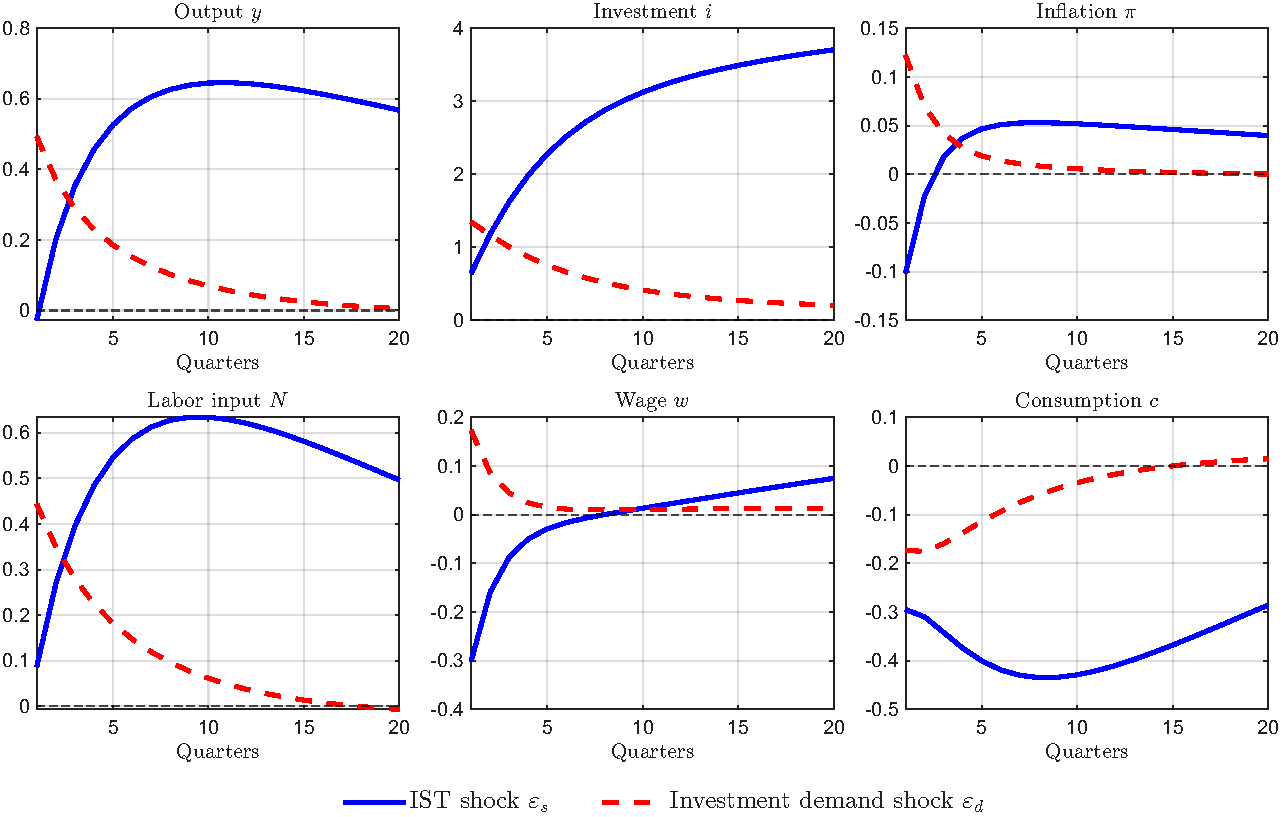
\includegraphics[width=0.9\textwidth]{figures/compare_irf_gov_data.pdf}
    \caption{Impulse responses of output, investment, inflation, labor input, wage, and consumption to one-standard-deviation IST and investment demand shocks (baseline estimation; horizon: 20 quarters).}
    \label{fig:compare_irf}
\end{figure}

Nevertheless, \cite{justinianoInvestmentShocksBusiness2010} uses the frequency based FEVD. To faciliate comparing, Table~\ref{tab:fevd-frequency:gov-data} shows the FEVD result based on the same methodology.

% Auto-generated by test_fevd_frequency.m
% file_name: gov_data
% band: 6--32 quarters; nbins=500

\begin{table}[!htbp]
\centering
\caption{Frequency-domain FEVD (\%) for the business-cycle band (6--32 quarters), with measurement error included (baseline estimation; 500 frequency bins).}
\label{tab:fevd-frequency:gov-data}
\begin{tabular}{l @{\hspace{2em}}r @{\hspace{2em}}r @{\hspace{2em}}r @{\hspace{2em}}r @{\hspace{2em}}r @{\hspace{2em}}r}
\hline\hline
Observable & $\varepsilon_g$ & $\varepsilon_{s}$ & $\varepsilon_R$ & $\varepsilon_a$ & $\varepsilon_{d}$ & $\mathrm{meas}$ \\ 
\hline
Output & 1.44 & 28.15 & 2.16 & 57.59 & 9.77 & 0.89 \\ 
Inflation & 0.13 & 16.26 & 17.73 & 59.52 & 5.06 & 1.29 \\ 
Interest rate & 0.16 & 22.76 & 9.76 & 58.55 & 6.33 & 2.45 \\ 
Hours & 2.68 & 49.48 & 1.49 & 23.25 & 16.69 & 6.42 \\ 
Investment & 0.19 & 54.18 & 0.18 & 28.69 & 15.72 & 1.03 \\ 
Gov. spending & 95.93 & 0.02 & 0.00 & 0.04 & 0.01 & 4.00 \\ 
\hline
\end{tabular}
\end{table}


The result shows that the aggregate technology has a much stronger effect on the business cycle, which accounts for about $50\%$ for output, inflation and nominal interest rate. IST shock contributes for $28.15\%$ of output, $16.26\%$ of inflation, $54.14\%$ of investment, and $49.48\%$ of hours worked. Meanwhile, investment demand shock is less important, accounting for $9.77\%$ of output, $5.06\%$ of inflation, $15.72\%$ of investment and $16.69\%$ of hours worked. 

Compared with the unconditional FEVD analysis in Table~\ref{tab:varcmp:gov-data}, the frequency FEVD restricts the impact to between 6 and 32 quarters. From the IRF plot in Figure~\ref{fig:compare_irf}, we can observe that the effect caused by investment demand shock almost converges to zero after 6 periods, which explains why it contributes less in frequency FEVD result.

\subsection{Inflation Impact}
\label{sec:results:inf}
Another interesting point in Figure~\ref{fig:compare_irf} is that the IST shock results in deflation in the first periods, while the investment demand shock generates inflation. Although this difference is documented in \cite{nireiOriginsPropagationAnimal}, which can be explained by the competition between substitution effect and wealth effect introduced before, \cite{justinianoInvestmentShocksBusiness2010} and Section \ref{sec:robustness} in this paper propose the contrary result---IST shock raises deflationary effect. Comparing the posterior, $\rho_{s}$ and $\psi_u$ show a big difference. Figure~\ref{fig:irf_rho_ist_psi_u_sign_flip} tests the inflation response to IST shock under various values of $\rho_{s}$ and $\psi_u$, where $\psi_u$ is defined from the household first-order condition of capital utilization rate \eqref{eq:util_foc},
$$\hat r^k_t = \frac{a''(1)}{a'(1)}\,\hat u_t \equiv \frac{\psi_u}{1 - \psi_u}\,\hat u_t.$$

\begin{figure}
    \centering
    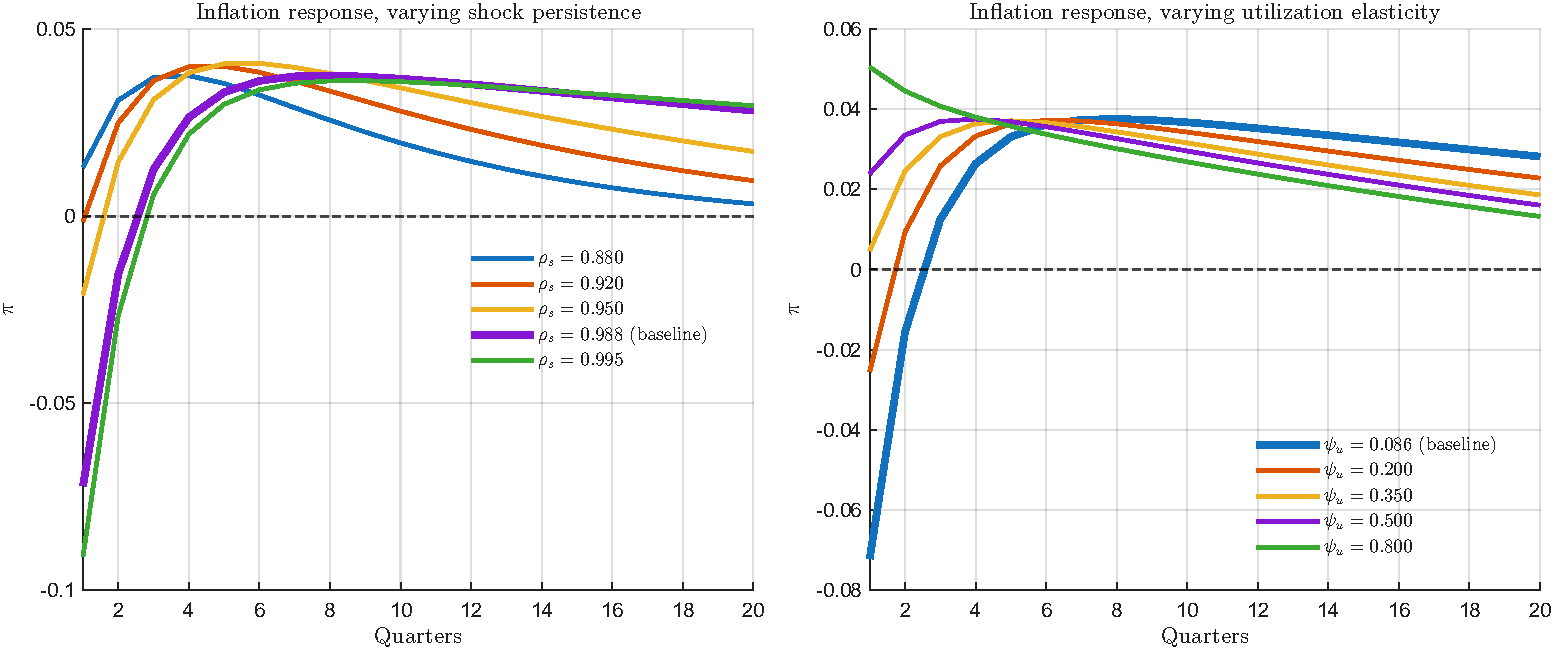
\includegraphics[width=0.7\textwidth]{figures/irf_rho_ist_psi_u_sign_flip.pdf}
    \caption{The sign of the inflation response to an IST shock depends on the estimated shock persistence $\rho_{s}$ and the capital-utilization elasticity $\psi_u$.}
    \label{fig:irf_rho_ist_psi_u_sign_flip}
\end{figure}

Under high $\rho_s$ and low $\psi_u$, the deflationary result is produced. However, inflationary result can be shown if $\rho_s$ is below $0.92$ or $\psi_u$ is above $0.32$,  keeping all other parameters unchanged. To understand the result, we can write the inflation as the summation of present discounted value of marginal cost,
\begin{equation}\label{eq:inf-mc}
    \hat{\pi}_t = \beta \mathbb{E}_t \hat{\pi}_{t+1} + \kappa_p \widehat{mc}_t \implies \hat{\pi}_t = \kappa_p \underbrace{\sum_{j = 0}^\infty \beta^j \mathbb{E}_t[\widehat{mc}_{t+j}]}_{= \, \text{PDV}(mc)}.
\end{equation}

Furthermore, there are two channel to influence the marginal cost---wage and capital rental rate, shown in Figure~\ref{fig:mc_decomposition_rk_psi_u}. The first shows that under low $\psi_u$, marginal cost is mainly accounted by the wage channel, while capital rental rate has only small effect in the first few periods. To understand this, we associate capital rental rate with firm's cost minimization decision \eqref{eq:loglin_factorprices} and households' capital utilization decision \eqref{eq:loglin_u},
\begin{equation}\label{eq:mpk-equal-rk}
    \begin{cases}
        \hat r^k_t = \hat w_t + \hat N_t - \hat K_{t-1} - \hat u_t\\
        \hat r^k_t = \frac{\psi_u}{1 - \psi_u}\,\hat u_t
    \end{cases}
    \implies
    \hat r^k_t = \psi_u \left(\hat w_t + \hat N_t - \hat k_{t-1}\right).
\end{equation}

\begin{figure}
    \centering
    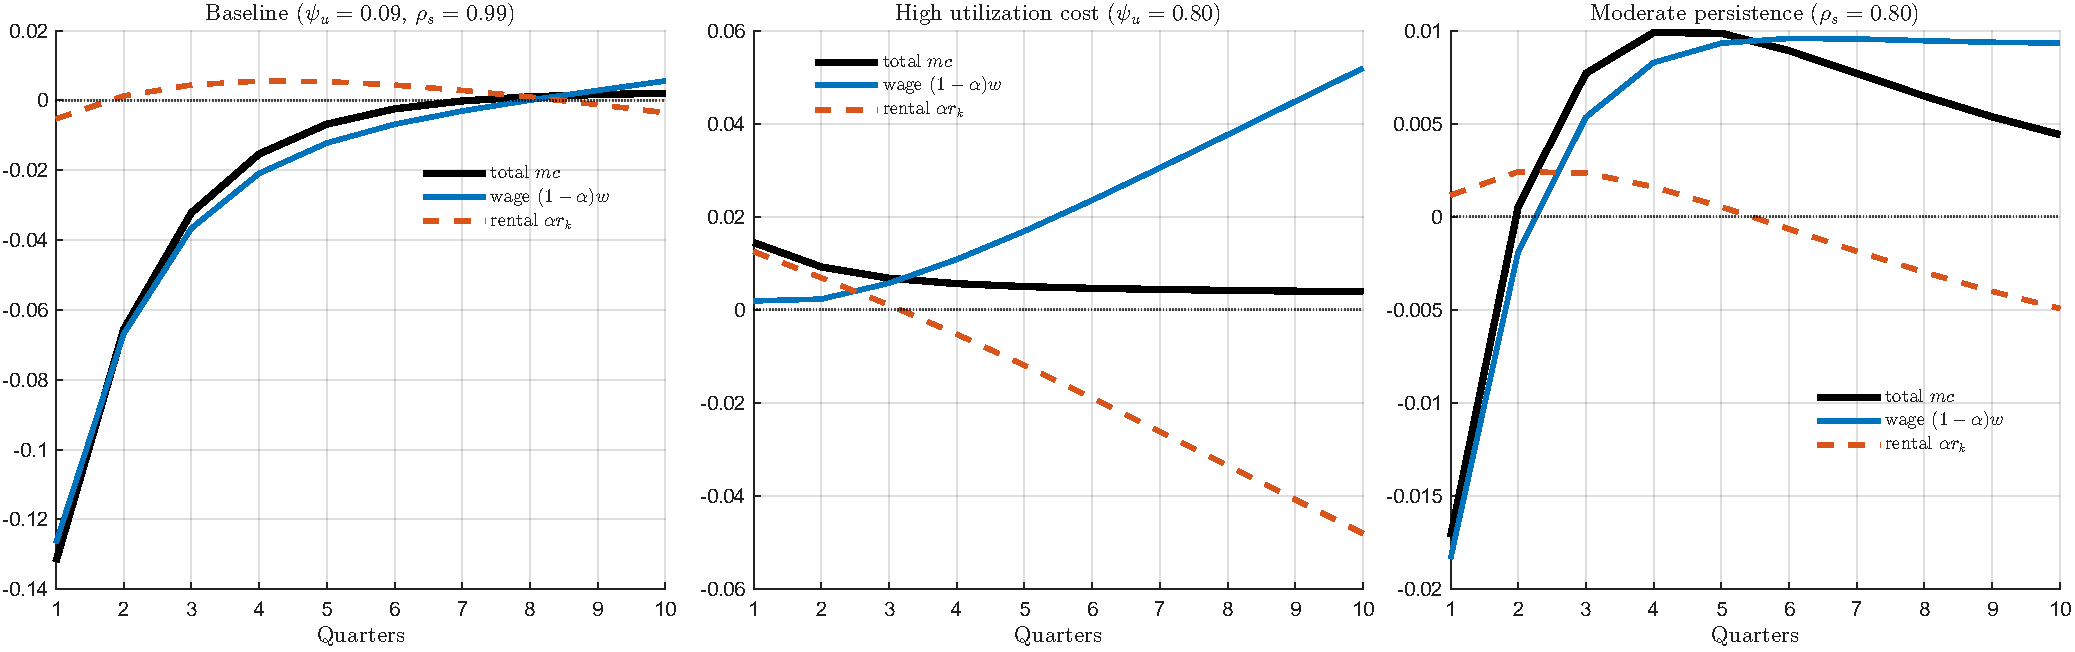
\includegraphics[width=0.9\textwidth]{figures/mc_decomposition_rk_psi_u.pdf}
    \caption{Decomposing the marginal-cost response to an IST shock: a wage channel against a capital-rental channel.}
    \label{fig:mc_decomposition_rk_psi_u}
\end{figure}

Equation \eqref{eq:mpk-equal-rk} shows $\hat r^k_t$ will only move $\psi_u$ fraction of $\hat w_t + \hat N_t$, as $\hat k_{t-1}$ is predetermined. First, under baseline result, $\hat w_t$ and $\hat N_t$ move to the opposite direction, which cancels out the absolute value of the difference. Second, the posterior of $\psi_u$ is only about $0.1$, dampening the magnitude a lot. However, the second panel of Figure~\ref{fig:mc_decomposition_rk_psi_u} shows the capital rental rate channel becomes important as $\psi_u$ becomes large, leading to the inflationary result. To understand this change, we can recall the definition of $\psi_u$ again. As $\frac{a''(1)}{a'(1)} = \frac{\psi_u}{1 - \psi_u}$, increase of $\psi_u$ implies $a''(1)$ becomes relatively larger. This means the adjustment cost function is steeper around the steady state. When the IST shock creates the increasing labor supply, marginal productivity of capital increases and thus capital demand increases. However, capital supply can hardly adjust due to the expensive adjustment cost. Therefore, the strong movement of the capital demand curve results in the high rental rate in the first few periods.

Understanding the role of $\psi_u$ helps the further analysis about $\rho_s$. Since $\psi_u$ is small in baseline posterior, we can focus on the wage channel. When $\rho_s$ decreases, the IST shock will persists shorter period once it arrives. Suppose IST shock is positive, then household will save more for shorter period when the investment is cheap, and thus wage will decrease for shorter time. As the current inflation is the summation of future marginal cost shown in equation~\eqref{eq:inf-mc}, it will be positive once the summation of negative initial terms is outweighed by the positive tail, as shown in the third panel of Figure~\ref{fig:mc_decomposition_rk_psi_u}.

It is worth stressing that the inflation impact under the IST shock is also sensitive to many other parameter values, such as the wage sticky parameter and the Phillips curve parameter, shown in Figure~\ref{fig:ist_sign_robustness}. Although the sign of the inflation impact is not robust to the parameter value choice, the sign of the wage impact shows a stable result in this exercise. However, I acknowledge the limitation of such an exercise: it alters parameters one by one, but cannot investigate the effect of simultaneous movement among several parameters. In fact, \cite{justinianoInvestmentShocksBusiness2010} shows the positive wage impact under IST shock.

\begin{figure}
    \centering
    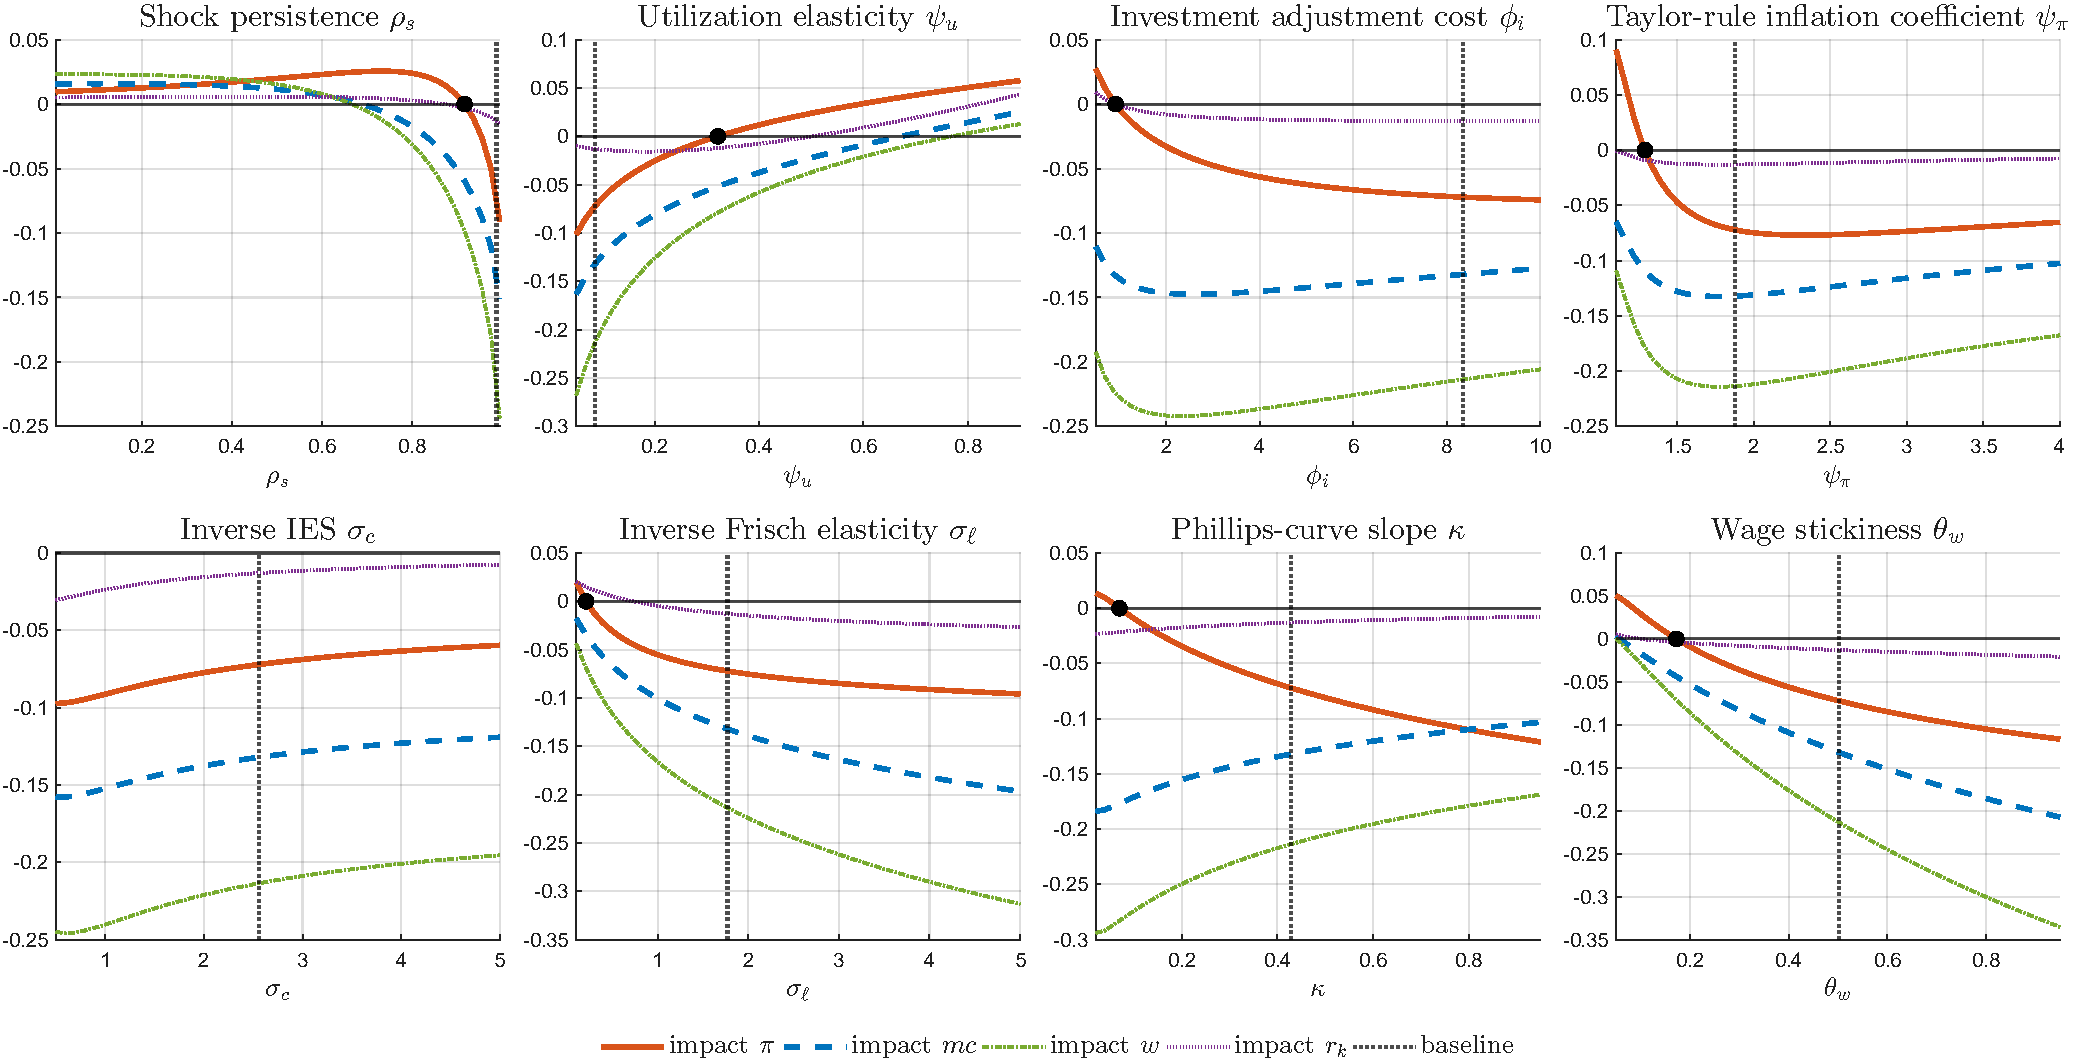
\includegraphics[width=\textwidth]{figures/ist_sign_robustness.pdf}
    \caption{Sensitivity of the sign of the impact inflation response to an IST shock. Each panel varies one parameter over a wide grid}
    \label{fig:ist_sign_robustness}
\end{figure}

On the other side, Figure~\ref{fig:inv_demand_mc_decomposition} shows the evidence about the robust inflationary effect of investment demand shock. The left panel shows both wage and capital rental rate increase under investment shock. This is because the shift of labor demand curve pushes up both labor input and wage, and thus capital rental rate increases by equation~\eqref{eq:mpk-equal-rk}. The right panel shows that the inflation impact is positive under the investment demand shock across all 500 selected draws. Moreover, as shown in Figure~\ref{fig:inv_demand_sign_robustnes}, the parameter sweep exercise confirms the robustness of this effect, and the wage impact remains positive during every single parameter sweep.

\begin{figure}
    \centering
    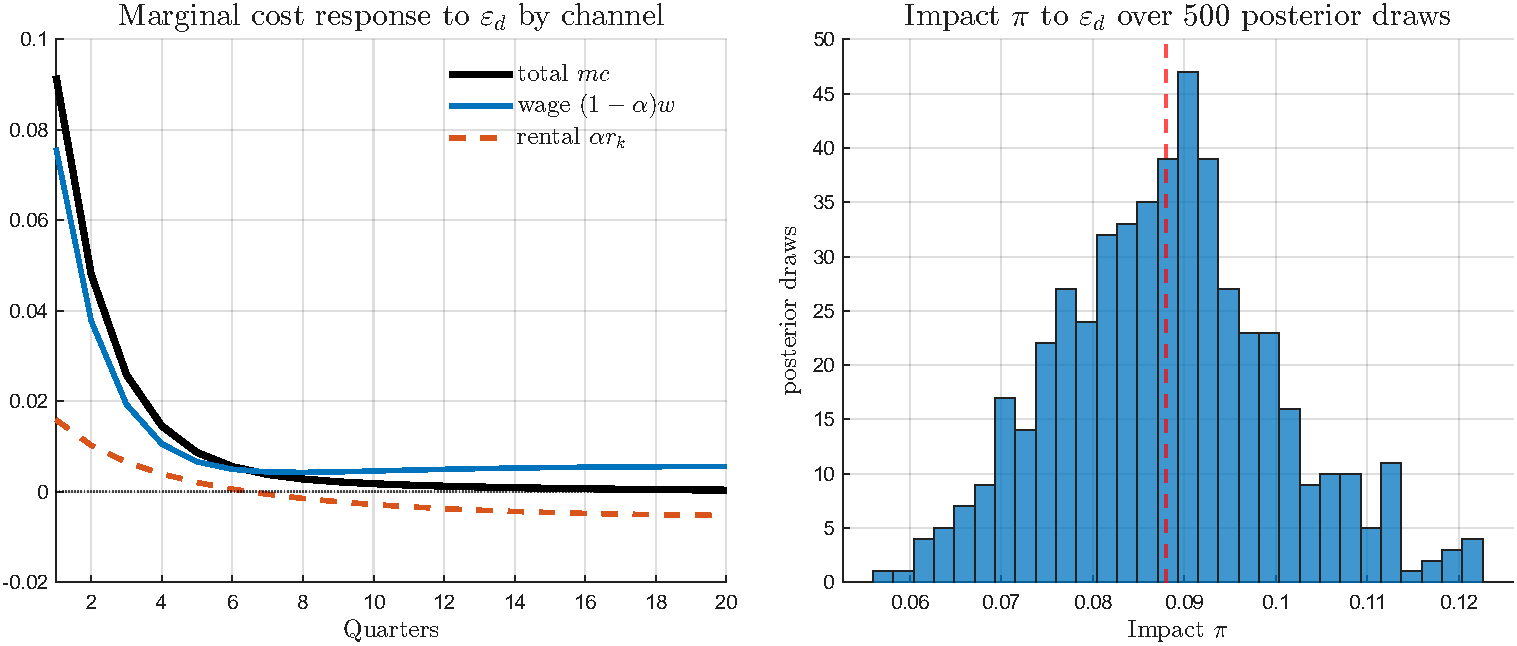
\includegraphics[width=0.7\textwidth]{figures/inv_demand_mc_decomposition.pdf}
    \caption{Robustness of the inflationary response to an investment-demand shock. \textit{Left panel.} Channel decomposition of the real marginal-cost response to a unit investment-demand shock at the baseline posterior mean. \textit{Right panel.} Impact inflation \(\hat\pi_1\) in response to a unit investment-demand shock across 500 posterior MH draws that are selected linarly across index among MH samples after burn-in.}
    \label{fig:inv_demand_mc_decomposition}
\end{figure}

\begin{figure}
    \centering
    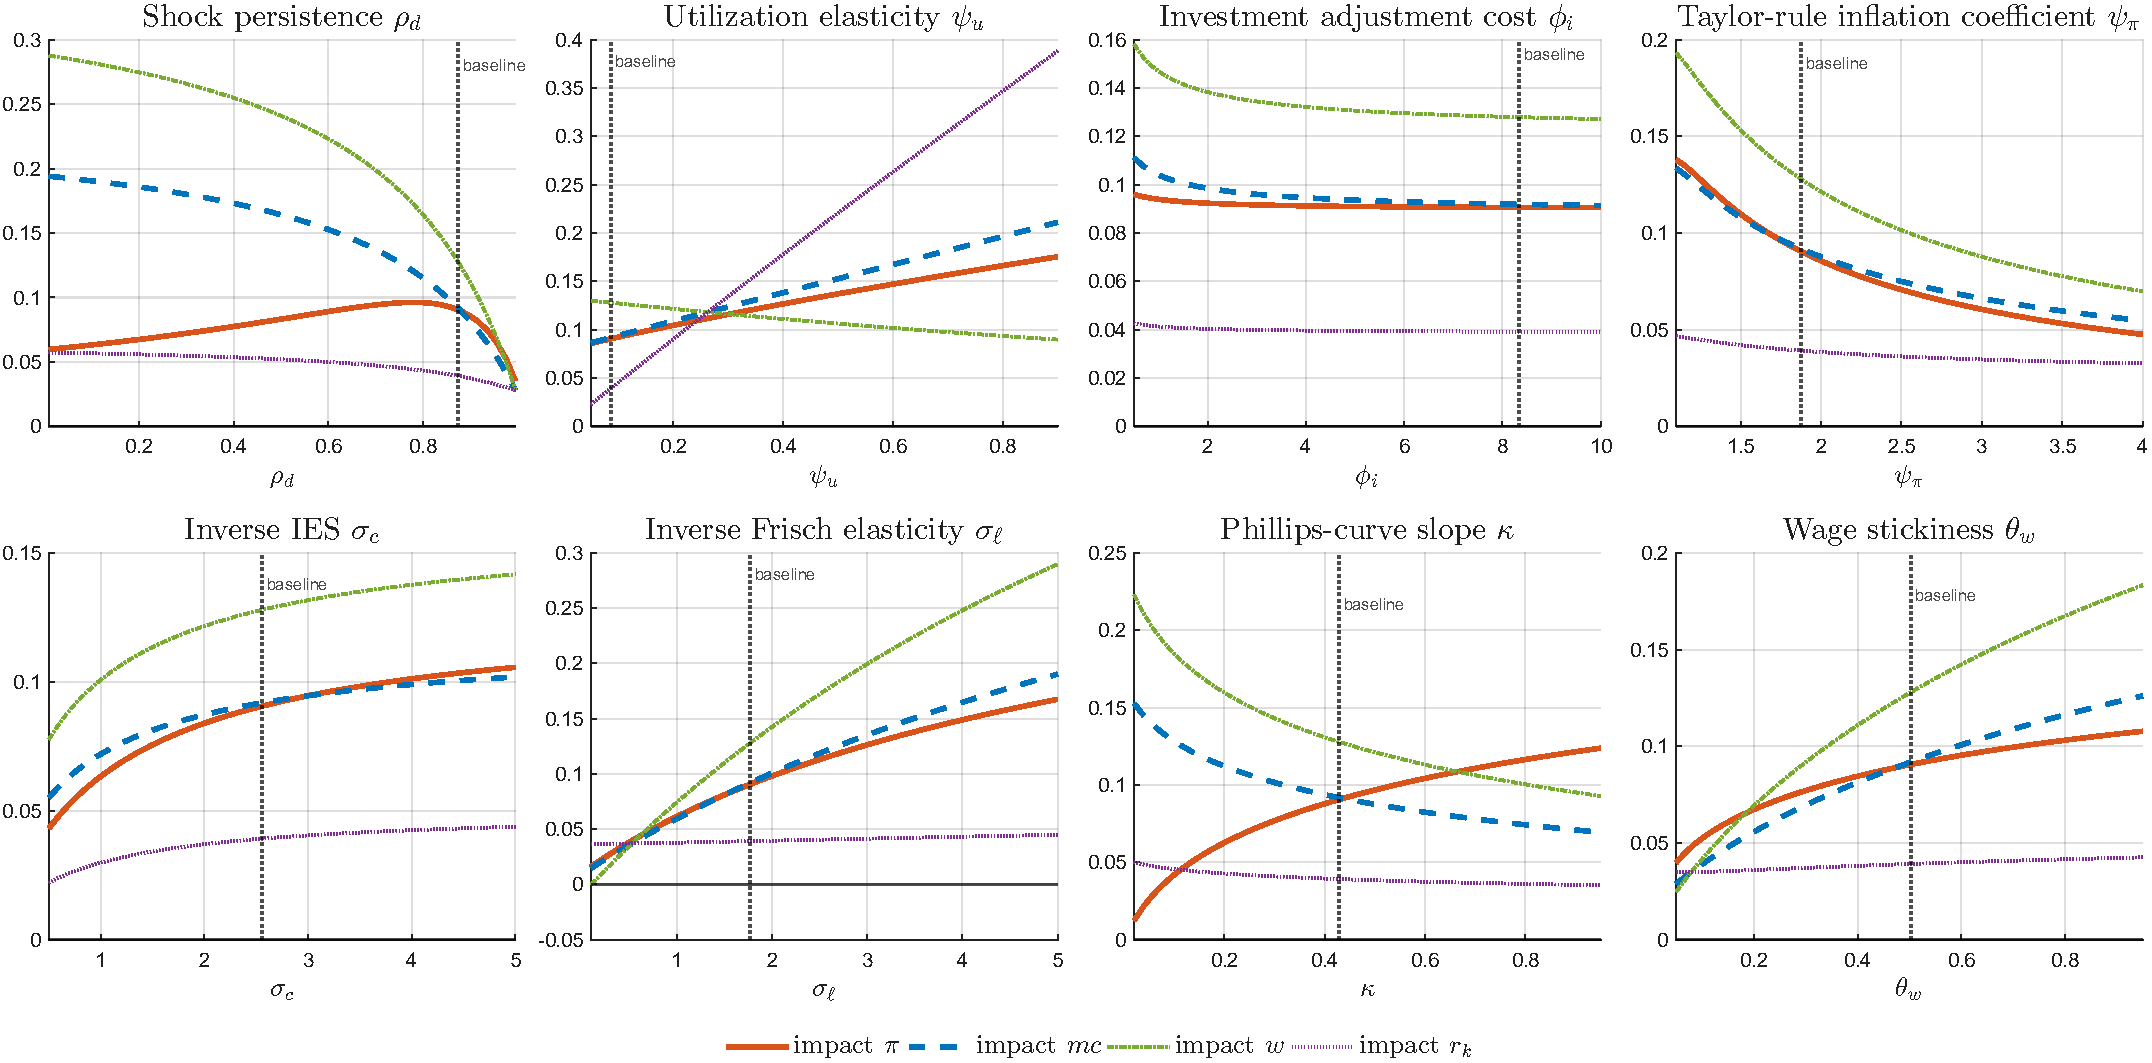
\includegraphics[width=\textwidth]{figures/inv_demand_sign_robustness.pdf}
    \caption{Robustness of the sign of the inflation response to an investment-demand shock. Each panel varies one parameter over a wide grid---the shock persistence \(\rho_d\), the capital-utilization elasticity \(\psi_u\), the investment adjustment cost \(\varphi_i\), and the Taylor-rule inflation coefficient \(\psi_\pi\)---holding all other parameters at the baseline posterior mean}
    \label{fig:inv_demand_sign_robustnes}
\end{figure}

\subsection{Consumption Impact}
\label{sec:results:con}
One of the attractions of the investment demand shock is its ability to generate comovements between consumption, investment and inflation, while the IST shock is usually unable to reproduce such a result. \cite{nireiOriginsPropagationAnimal} shows that the positive comovement shows up under certain calibrations, and one of the quests of this paper is to test whether the estimation supports such a result.

However, as shown in the IRF plot, Figure~\ref{fig:compare_irf}, the consumption impact is negative. Moreover, altering a single parameter value cannot reproduce a positive consumption impact either---such a result relies on certain parameter combinations. To figure out which parameter combination is needed, I align some model settings to \cite{nireiOriginsPropagationAnimal}, and simultaneously change three parameters that are important in theoretical proof---Phillips-curve slope \(\kappa_p\), the Taylor-rule inflation coefficient \(\psi_\pi\) and the wage-rigidity parameter \(\theta_w\). Result in Figure~\ref{fig:inv_demand_c1_kappa_psipi_heatmap} shows that, generally, if all three parameters are low enough, then consumption impact can be positive \footnote{Some may question about the indeterminate area in Figure~\ref{fig:inv_demand_c1_kappa_psipi_heatmap}, since the textbook new Keyasian model can be uniquely solven once $\psi_\pi > 1$. However, the problem becomes more complicated when capital and investment are added into the model, and \cite{sveen2005new} provides a detailed theoretical analysis about it.}. 

\begin{figure}
    \centering
    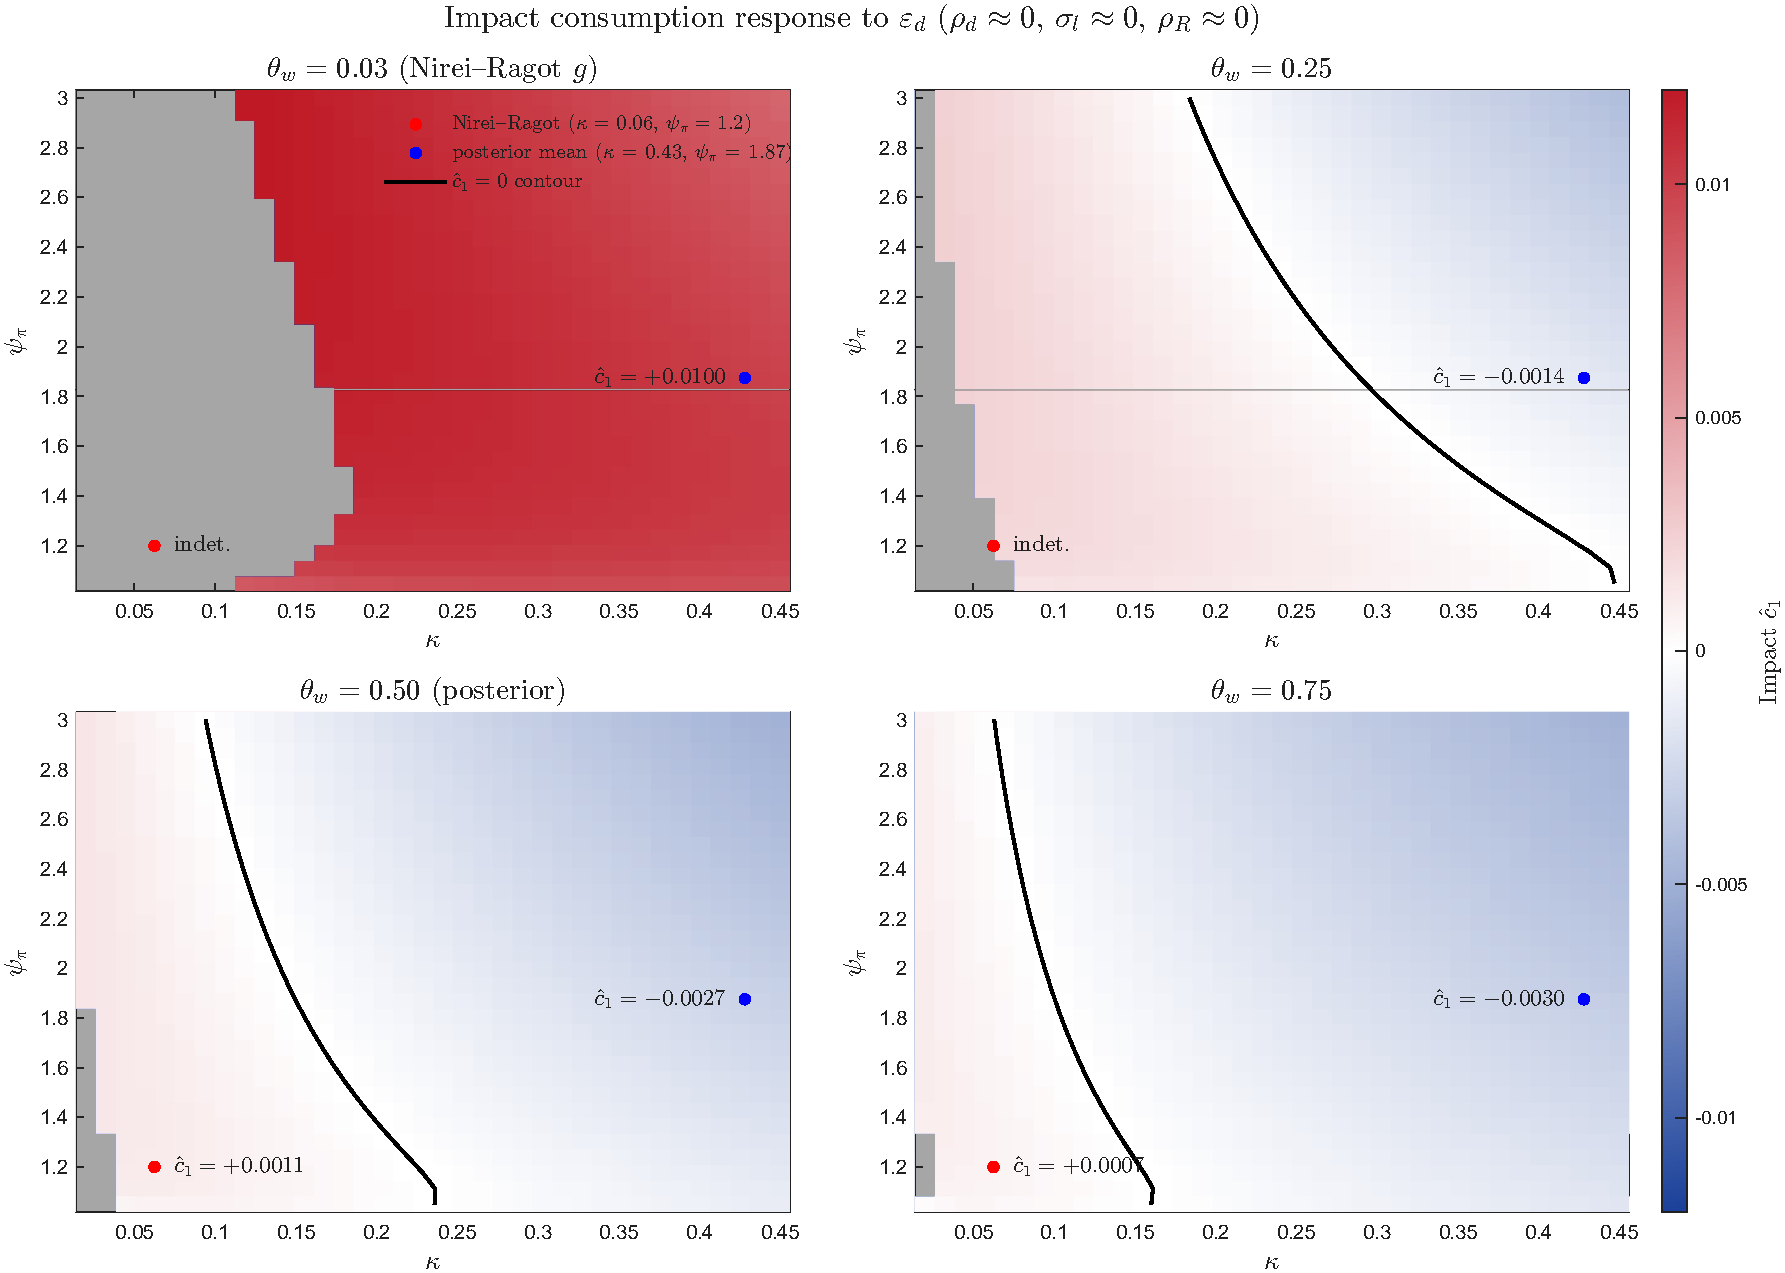
\includegraphics[width=\textwidth]{figures/inv_demand_c1_kappa_psipi_heatmap.pdf}
    \caption{Impact consumption response \(\hat c_1\) to a unit investment-demand shock as a function of the Phillips-curve slope \(\kappa_p\) and the Taylor-rule inflation coefficient \(\psi_\pi\) four values of the wage-rigidity parameter \(\theta_w\). The remaining parameters are held at the calibration in \cite{nireiOriginsPropagationAnimal}: an i.i.d. shock (\(\rho_d \approx 0\)), a non-inertial pure-inflation rule (\(\rho_R\approx 0\)), and near-linear labor disutility (\(\psi \approx 0\)). Gray cells are indeterminate configurations.}
    \label{fig:inv_demand_c1_kappa_psipi_heatmap}
\end{figure}

The result can be understand as follows. In short run, investment demand shock pushes up aggregate demand, but in long run accumulating more capital. Instead of investment, imagine that the capital increases directly. This simply makes households more wealthy, and thus they will consume more today. So, how to let the investment demand shock be analogous to direct capital increase? We can shut down the short-run effect by letting the economy to be more sticky---lower $\theta_w$ suppressing wage, lower $\kappa_p$ suppressing inflation, and lower $\psi_\pi$ suppressing nominal interest rate. They can then form a chain to suppress intertemporal substitution effect. If the wage increases only mildly, marginal cost will not increase much; if the Phillips curve is flat, inflation will not increase much; and if the Taylor rule is inactive to inflation, then the nominal interest rate will be stable; finally, since the real interest rate is stable, households will not shift today's consumption to tomorrow.

\subsection{Historical Decomposition}
\label{sec:results:hd}
To investigate the shock effects along the historical data, I show the historical decomposition in Figure~\ref{fig:hd:gov_data}, where the fluctuation of the fundamental macroeconomic data are decomposed into the fluctuation of structural shocks.

\begin{figure}
    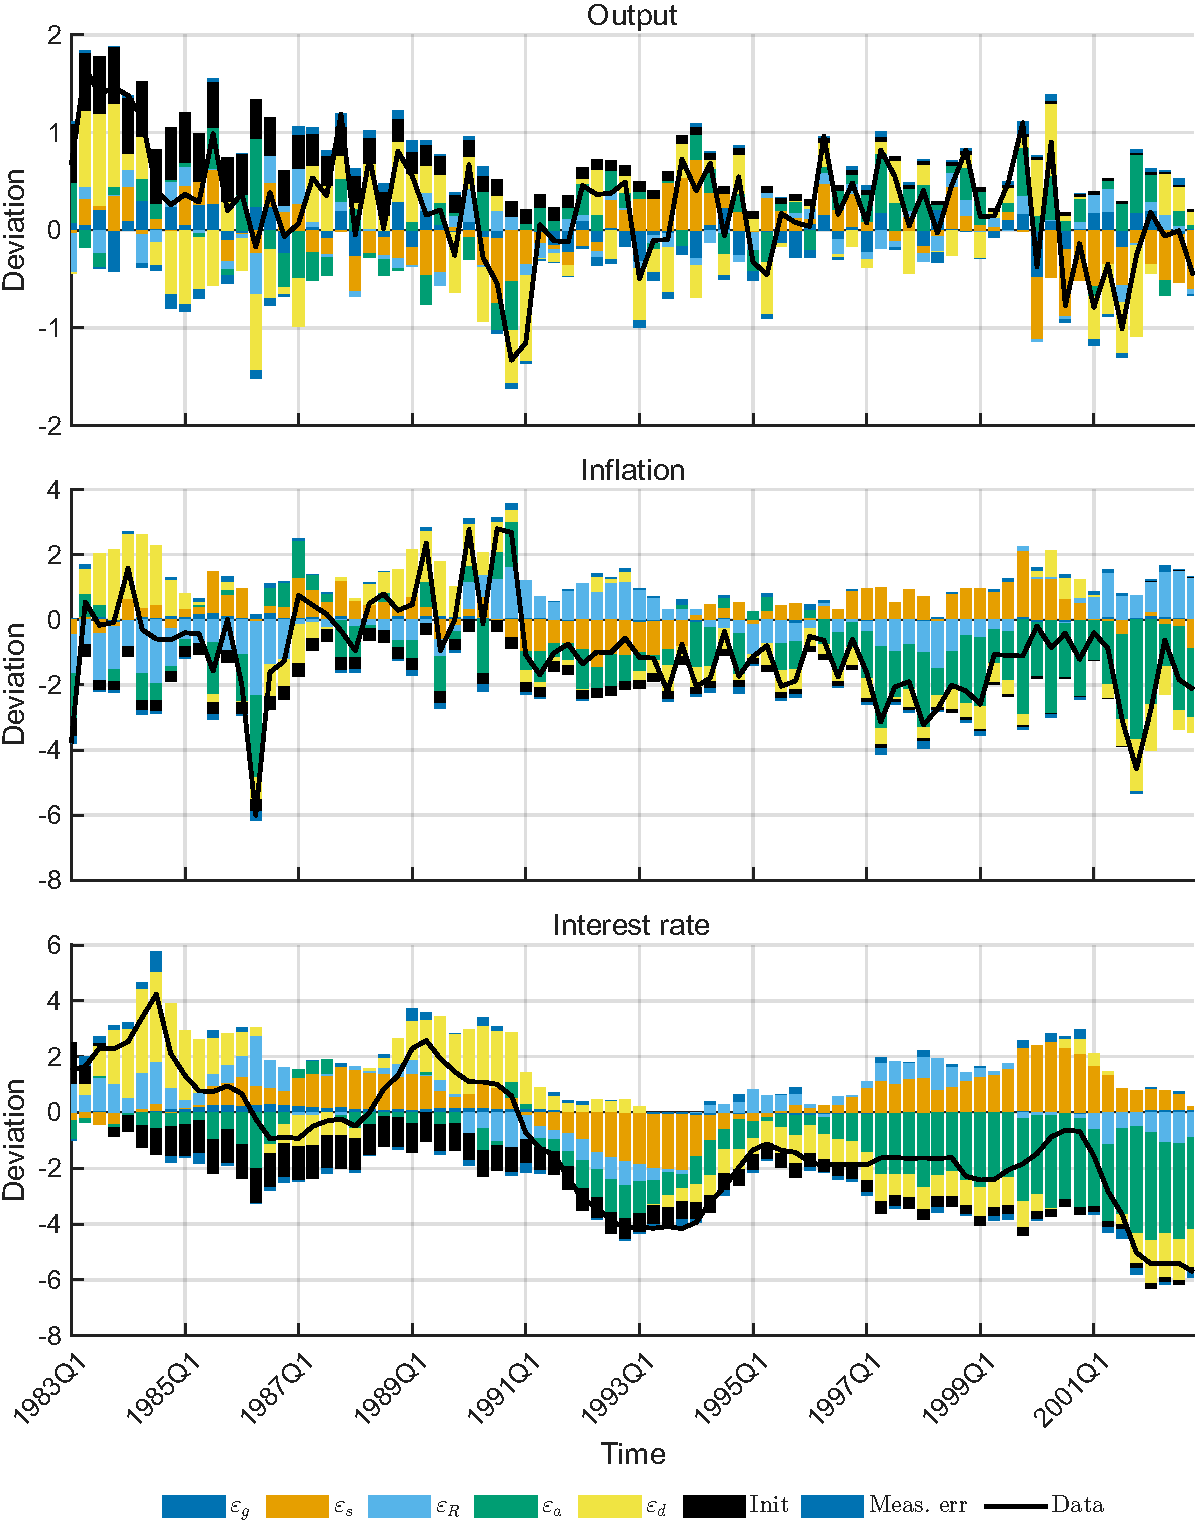
\includegraphics[width=0.9\textwidth]{figures/hd_gov_data.pdf}
    \caption{Historical decomposition (Kalman smoother) of demeaned output growth, inflation, and nominal interest rate into contributions from structural shocks (including initial conditions and measurement error) in the estimated baseline model.}
    \label{fig:hd:gov_data}
\end{figure}

Compared with the IST shock, the investment demand shock is shown to be more volatile in the HD of output, which often switches direction from quarter to quarter. Also, it behaves more procyclically, nearly moving in the same direction as output and inflation.

During the oil crisis in 1990-1991, both the IST shock and the investment demand shock show a very negative influence on output. After 1995, the aggregate productivity shock becomes the main driving force of inflation and the nominal interest rate. 

\section{Robustness Test}
\label{sec:robustness}
Three alternative settings are used to test the baseline result regarding the investment demand shock---the first one uses the standard \cite{smetsShocksFrictionsUS2007} model; the second discusses the case where the investment demand shock is i.i.d.; the last one further differentiates the IST shock and the marginal efficiency of investment (MEI) shock, following \cite{justinianoInvestmentShocksRelative2011}.

\subsection{Smets--Wouters-style Model}
\label{sec:robustness:sw}
In this section, the baseline model is expanded following \cite{smetsShocksFrictionsUS2007} to address the underlying concerns of oversimplification. Specifically, I add a habit formation term in the utility function and a monopolistic competition structure in the labor market. In addition, a preference shock, a price markup shock and a wage markup shock are added as well. In terms of data, the consumption and wage growth rates are added.

The utility function of households becomes
\begin{equation}
    \mathbb{E}_t \left[ \sum_{s=0}^{\infty} \beta^s \mu_{b, t+s} \left( \ln(C_{t+s} - h C_{t+s-1}) - \chi \frac{L_{t+s}(j)^{1+\psi}}{1+\psi} \right) \right],
\end{equation}
where $\mu_{b, t}$ is the intertemporal preference shock, following
\begin{equation}
    \ln \mu_{b, t} = (1 - \rho_b) \mu_b + \rho_b \ln \mu_{b, t-1} + \varepsilon_{b, t}, \,\, \varepsilon_{b, t}\sim \text{i.i.d. } N (0, \sigma_b^2).
\end{equation}

It is worth to mention that the consumption part in the utility function becomes logarithmic instead of the more general CRRA form. This is because with habit formation and separable utility function between $C_t$ and $L_t$, general CRRA utility function doesn't have a balanced growth path unless it reduces to a logarithmic form.

The stochastic discount factor becomes
\begin{equation}
    SDF_t = \beta \left(\frac{c_{t+1} - hc_t}{c_t - hc_{t-1}}\right)^{-1} = \beta \left(\frac{\gamma \tilde{c}_{t+1} - h\tilde{c}_t}{\tilde{c}_t - \frac{h}{\gamma}\tilde{c}_{t-1}}\right)^{-1},
\end{equation}
where $\tilde{c}_t = c_t / \gamma^t$ is the detrended variable.

The labor market and wage Calvo pricing problem follow \cite{erceg2000optimal}, which gives us the wage Phillips curve
\begin{equation}
    \hat{\pi}_t^w = \beta \mathbb{E}_t \hat{\pi}_{t+1}^w - \kappa_w \left(\hat{w}_t - \hat{MRS}_t\right) + \mu_{w, t},
\end{equation}
where $\kappa_w = \frac{(1 - \theta_w)(1 - \beta\theta_w)}{\theta_w(1+\nu_{w} \psi)}$. Because of the weak identification problem \footnote{$\nu_w$, $\theta_w$ only play a role in $\kappa_w$, but $\kappa_w$ can be the same under different value combinations of $\nu_w$ and $\theta_w$. Thus the model will be unable to identify $\nu_w$ and $\theta_w$ parameters separately.}, $\nu_w$ is set as $3$ following \cite{smetsShocksFrictionsUS2007}.

$\mu_{w, t}$ is the wage markup shock following
\begin{equation}
    \ln \mu_{w, t} = (1 - \rho_w) \mu_w + \rho_w \ln \mu_{w, t-1} + \varepsilon_{w, t}, \,\, \varepsilon_{w, t}\sim \text{i.i.d. } N (0, \sigma_w^2).
\end{equation}

The price markup shock $\mu_{p, t}$ is added in the same way---right after the Phillips curve. I assume the markup shocks follow AR(1) processes for simplicity, while \cite{smetsShocksFrictionsUS2007} uses ARMA(1, 1) processes for these two shocks.

Two added observation equations are
\begin{equation}
    \begin{bmatrix}
        \Delta \ln CONS_t\\
        \Delta \ln WAGE_t
    \end{bmatrix}
    = 
    \begin{bmatrix}
        \bar{\gamma}\\
        \bar{\gamma}
    \end{bmatrix}
    +
    \begin{bmatrix}
        \hat{c}_t - \hat{c}_{t-1} \\
        \hat{w}_t - \hat{w}_{t-1}
    \end{bmatrix}
    +
    \Sigma_t^{meas}.
\end{equation}

Posteriors can be found in Table~\ref{tab:posterior-params:sw-type-no-rel} in Appendix \ref{app:result:sw}. Especially, both the Phillips curve and the wage Phillips curve become very flat, with $\kappa_p$ estimated as $0.03$ and $\kappa_w$ roughly $0.02$, which are much stickier than in the baseline result. A simple test that mutes the price and wage markup shocks shows that the low $\kappa_p$ and $\kappa_w$ partially benefit from these shocks, as they can alter price and wage exogenously, even though the endogenous part is rather sticky. The moments comparison is shown in Table~\ref{tab:varcmp:sw-type-no-rel}. As explained in Section~\ref{sec:results:moments}, the variance of hours worked is fitted much better.

It is clear that the investment demand shock has only a marginal effect on various macroeconomic variables, as shown in Table~\ref{tab:vd:sw-type-no-rel}. The investment demand shock can only contribute $4.37\%$ of the output forecast variance and $13.62\%$ of investment, and can hardly explain other variables such as inflation. Thus I flag the fragility of the baseline result in Table~\ref{tab:fevd-frequency:gov-data}.

% Auto-generated by test_variance_decomp_nocap.m
% file_name: sw_type_no_rel

\begin{table}[!htbp]
\centering
\caption{Unconditional FEVD (\%): Smets--Wouters-style model.}
\label{tab:vd:sw-type-no-rel}
\begin{tabular}{l r r r r r r r r}
\hline
Observable & $\varepsilon_g$ & $\varepsilon_{s}$ & $\varepsilon_R$ & $\varepsilon_a$ & $\varepsilon_b$ & $\varepsilon_p$ & $\varepsilon_w$ & $\varepsilon_{d}$ \\ 
\hline
Output & 6.15 & 10.31 & 7.86 & 43.58 & 17.21 & 5.00 & 5.52 & 4.37 \\ 
Inflation & 0.05 & 1.78 & 0.82 & 18.85 & 0.40 & 53.05 & 25.04 & 0.00 \\ 
Interest rate & 0.19 & 7.16 & 30.37 & 26.67 & 4.51 & 10.39 & 20.72 & 0.00 \\ 
Hours & 2.00 & 20.43 & 7.10 & 34.85 & 7.86 & 1.10 & 26.35 & 0.30 \\ 
Investment & 0.25 & 54.98 & 2.43 & 18.59 & 3.19 & 0.62 & 6.33 & 13.62 \\ 
Wage & 0.00 & 0.12 & 0.14 & 18.25 & 0.30 & 16.96 & 64.23 & 0.00 \\ 
Consumption & 0.25 & 2.36 & 6.48 & 43.49 & 42.01 & 1.92 & 3.49 & 0.00 \\ 
Gov. spending & 99.90 & 0.01 & 0.01 & 0.05 & 0.02 & 0.01 & 0.01 & 0.00 \\ 
\hline
\end{tabular}
\end{table}


Figure~\ref{fig:irf:sw} plots the IRF of the same state variables with the IRF of baseline result. There are three points that are different from the baseline result in Figure~\ref{fig:compare_irf}. First, investment demand shock generates much less fluctuation than IST shock due to the smaller standard deviation; second, IST shock now generates inflationary result, and the positive wage impact as well; third, consumption impact under investment demand shock becomes smoother---consumption impact is only $0.2\%$ of investment impact, whereas it is $12\%$ in the baseline result.

\begin{figure}
    \centering
    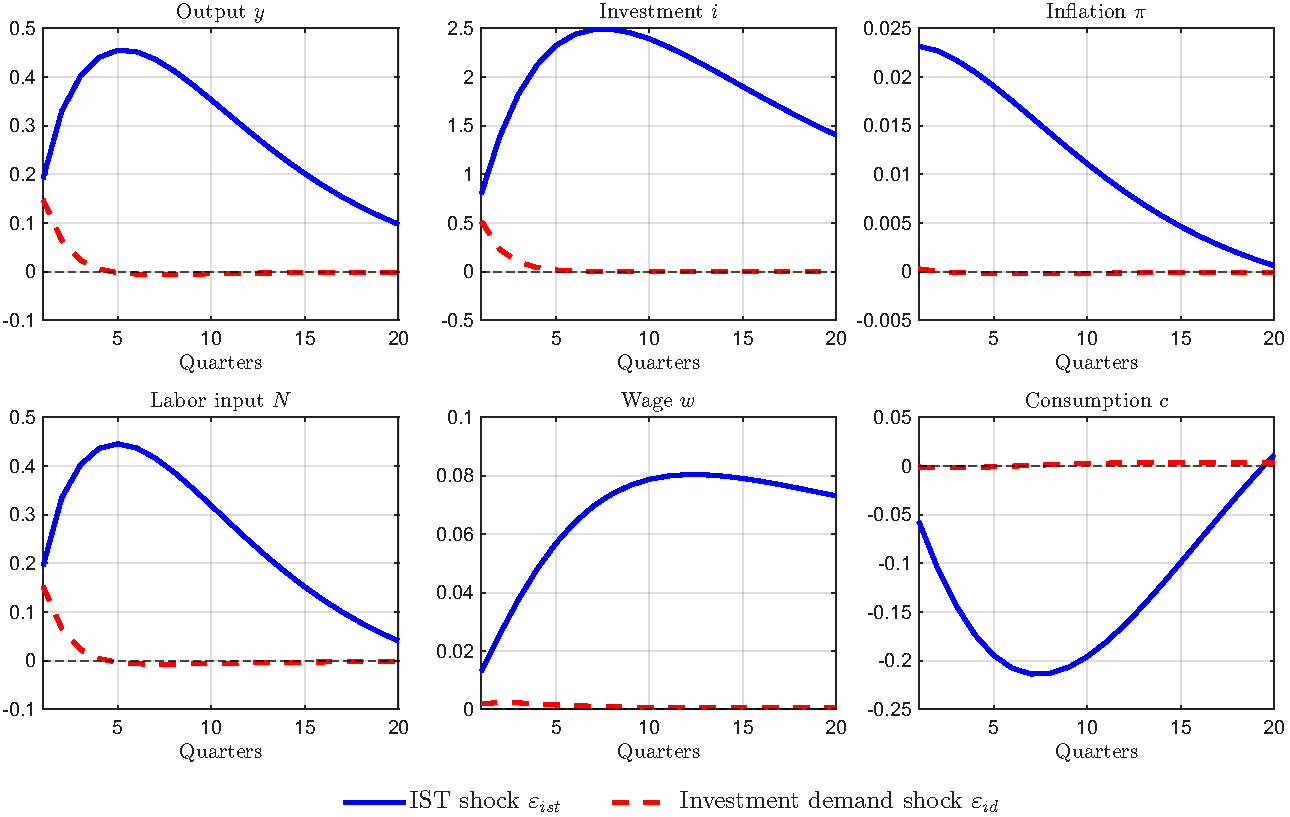
\includegraphics[width=0.9\textwidth]{figures/compare_irf_sw_type_no_rel.pdf}
    \caption{Impulse responses of output, investment, inflation, labor input, wage, and consumption to one-standard-deviation IST and investment demand shocks (Smets--Wouters-style model; horizon: 20 quarters).}
    \label{fig:irf:sw}
\end{figure}

I revisit the consumption impact in Figure~\ref{fig:sw:con}. Compared with the similar exercise in baseline result (Figure~\ref{fig:inv_demand_c1_kappa_psipi_heatmap}), I choose the parameters, the inverse Frisch elasticity $\psi$ and Taylor-rule output-gap coefficient $\psi_y$, to be varied. This is because the Phillips curve, as well as the wage Phillips curve, becomes quite flat. Thus, the slopes themselves have already approached to the \cite{nireiOriginsPropagationAnimal} calibration, and further, the inflation feedback in the Taylor's rule becomes less important because inflation hardly moves. However, the logic keeps the same---consumption impact is decided by the path of real interest rate, so nominal interest rate helps. If nominal interest rate is low enough, real interest can also be very low, and thus intertemporal substitution effect will be tempered. Smaller $\psi_y$ explicitly does this job by lowering output gap feedback in Taylor's rule. Smaller $\psi$ works through the output gap by suppressing the real wage---because nominal wage is very stikcy, the wage gap is smaller if real wage barely moves, and thus the output gap becomes smaller.
\begin{figure}
    \centering
    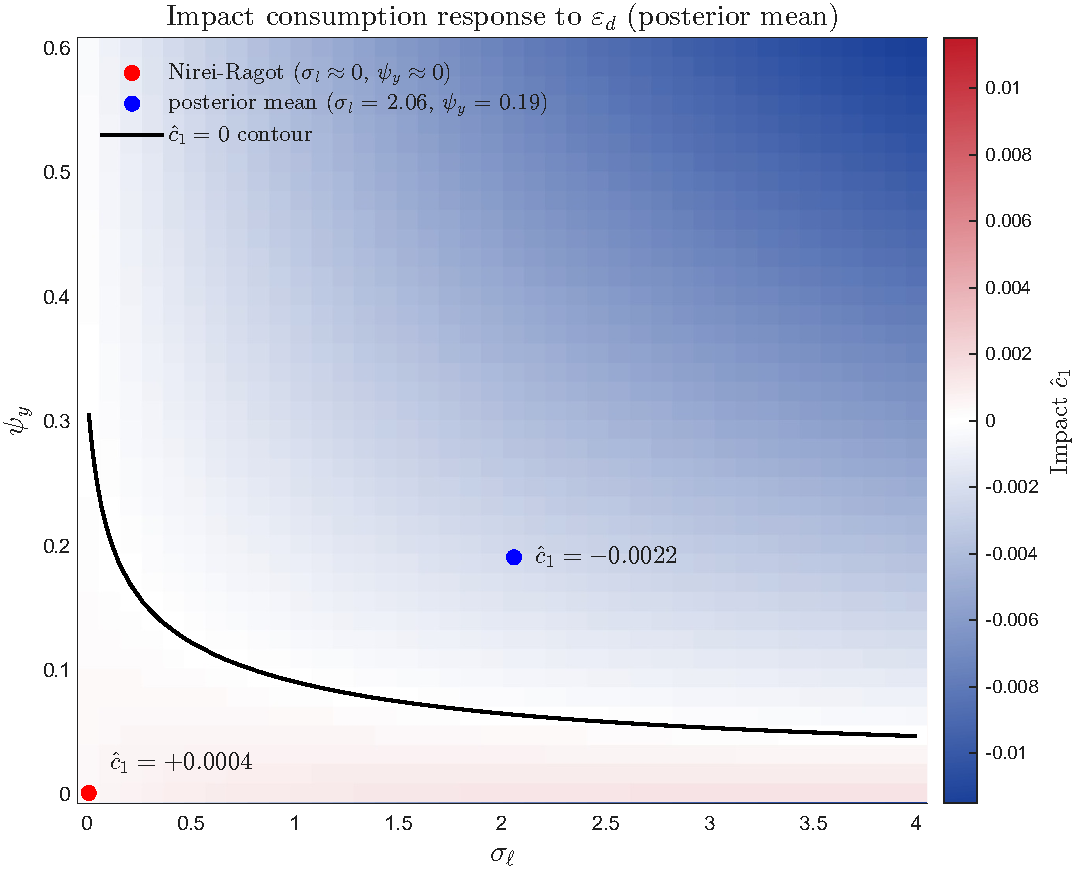
\includegraphics[width=0.7\textwidth]{figures/inv_demand_c1_psiy_sigmal_heatmap.pdf}
    \caption{Impact consumption response \(\hat c_1\) to a unit investment-demand shock as a function of the inverse Frisch elasticity \(\psi\) and the Taylor-rule output-gap coefficient \(\psi_y\). All other parameters are held at the posterior mean. }
    \label{fig:sw:con}
\end{figure}

Altogether, this section shows the sensitivity of the baseline result under an alternative model setting. However, its result can still be understood from the mechanisms analyzed in Section~\ref{sec:results}.

\subsection{Independent Investment Demand Shock}
\label{sec:robustness:iid}
Although using an AR(1) process to specify shocks is standard, it is natural to think that households will realize the exogenous investment demand in the $t+1$ period, and thus adjust their investment decision in $t+1$ to dampen the effect of the investment demand shock. Equivalently, this is to say that the investment demand shock only has a transitory effect in period $t$, which motivates the exercise in this section.

All other settings are unchanged compared with the baseline, except that $\rho_d$ is manually set as $0$. To be concise, I only present the FEVD result here in Table~\ref{tab:varcmp:per-add-mei}, and others can be found in Table~\ref{tab:posterior-params:per-add-mei} and Table~\ref{tab:varcmp:per-add-mei} in Appendix~\ref{app:result:iid}.

% Auto-generated by test_variance_decomp_nocap.m
% file_name: per_add_mei

\begin{table}[!htbp]
\centering
\caption{Variance decomposition (\%).}
\label{tab:vd:per-add-mei}
\begin{tabular}{l r r r r r}
\hline
Observable & $\varepsilon_g$ & $\varepsilon_{s}$ & $\varepsilon_R$ & $\varepsilon_a$ & $\varepsilon_{d}$ \\ 
\hline
Output & 6.67 & 38.60 & 9.35 & 22.42  & 22.95 \\ 
Inflation & 0.40 & 52.00 & 12.87 & 34.37 & 0.37 \\ 
Interest rate & 0.37 & 74.14 & 3.74 & 21.66 & 0.09 \\ 
Hours & 2.84 & 92.22 & 0.12 & 4.53 & 0.29 \\ 
Investment & 0.25 & 73.06 & 0.20 & 11.31 & 15.18 \\ 
Gov. spending & 99.59 & 0.17 & 0.04 & 0.10 & 0.10 \\ 
\hline
\end{tabular}
\end{table}


The investment demand shock contributes $22.95\%$ of output and $15.18\%$ of investment forecast error variance. Compared with the baseline result in Table~\ref{tab:fevd-frequency:gov-data}, the influence of the investment demand shock also decreases as expected, since the zero persistence cuts off the future influence.

\subsection{Marginal Efficiency of Investment Shock}
\label{sec:robustness:mei}
The topic in this section is subtle---it further distinguishes the IST shock from the marginal efficiency of investment (MEI) shock. Specifically, the IST shock means the efficiency from consumption goods to investment goods, and the MEI shock means the efficiency from investment goods to capital. However, without modelling the detailed investment goods producers and capital producers, both shocks stay in the capital law of motion in their reduced form,
\begin{equation}\label{eq:mei}
    k_{t+1} = (1 - \delta) k_t + \mu_{s, t}\mu_{m, t}\left[1 - S\left(\frac{i_t}{i_{t-1}}\right)\right] i_t,
\end{equation}
and thus there will be weak identification problem within the previous data set.

This test is motivated by \cite{justinianoInvestmentShocksRelative2011}, who claim that the IST shock will become less important if it is identified by data, and that the MEI shock becomes the one that matters. However, this raises a doubt about the estimation result---is the important thing just the residual in the capital law of motion? Although we can write multiple shocks in the capital law of motion, the equation suffers from a misspecification problem, in that we cannot be sure what the real shocks are. We can claim an IST shock, an investment demand shock, or an MEI shock in the capital law of motion, but which shocks to add depends on our assumptions. If the data-identified shock is less important, then the other part may be just the residual in the equation, and it is significant no matter what shock is named.

To alleviate the concern, the best thing to do is to identify the investment shock directly by some data. However, as this shock originates from idiosyncratic productivity shocks, the micro data that we need can hardly be incorporated into the current framework, where we only consider aggregate variables. Therefore, I can only conduct a horse-race test in this section by adding the MEI shock into the model. The result cannot conclusively establish the importance of the investment demand shock, but only offer some suggestions.

I use the relative price data to solve the weak identification problem mentioned in equation \eqref{eq:mei}. As pointed out by \cite{greenwoodLongRunImplicationsInvestmentSpecific1997a} and \cite{fisherDynamicEffectsNeutral2006}, the relative price of investment reflects the investment specific technology level in a one-sector model \footnote{If we model the production of consumption goods and investment goods as two sectors, such as in \cite{mouraInvestmentShocksSticky2018}, the relative price of investment goods is represented as the relative productivity, markup and marginal cost between these two sectors. Therefore, the relative price should have more complex dynamics in a more realistic model, rather than being only an exogenous stochastic process.}. Therefore, using the detrended relative price data, I assume that the detrended relative price represents the inverse of the IST level state variable. The data, the relative price of investment goods (PIRIC), is collected from FRED, and then I take $100\ln PIRIC_t$. As the data has an obvious trend, it should be detrended to match the model assumption that the logarithm of the IST level is a stationary process. Although it is more realistic to model the logarithm of IST level as a random walk process given the data, such modeling requires recalculating the balanced growth path, steady state and log-linearized model, as another growth term is added into the model. Thus, using the detrended data is a more straightforward approach.

% Auto-generated by test_variance_decomp_nocap.m
% file_name: para_add_mei

\begin{table}[!htbp]
\centering
\caption{Variance decomposition (\%).}
\label{tab:vd:para-add-mei}
\begin{tabular}{l r r r r r r}
\hline
Observable & $\varepsilon_g$ & $\varepsilon_{s}$ & $\varepsilon_R$ & $\varepsilon_a$ & $\varepsilon_{m}$ & $\varepsilon_{d}$ \\ 
\hline
Output & 4.58 & 0.44 & 10.81 & 23.79 & 17.22 & 43.16 \\ 
Inflation & 0.31 & 0.78 & 10.33 & 34.79 & 47.64 & 6.15 \\ 
Interest rate & 0.35 & 1.31 & 4.77 & 25.98 & 61.45 & 6.14 \\ 
Hours & 3.01 & 0.44 & 0.08 & 3.01 & 92.01 & 1.45 \\ 
Investment & 0.12 & 1.09 & 0.17 & 11.10 & 38.88 & 48.63 \\ 
Gov. spending & 99.65 & 0.00 & 0.04 & 0.09 & 0.06 & 0.16 \\ 
Relative price & 0.00 & 100.00 & 0.00 & 0.00 & 0.00 & 0.00 \\ 
\hline
\end{tabular}
\end{table}


Table \ref{tab:vd:para-add-mei} reports the FEVD in the model incorporating the MEI shock and relative price data, and other results are shown in Table~\ref{tab:posterior-params:para-add-mei} and Table~\ref{tab:varcmp:para-add-mei} in Appendix~\ref{app:result:mei}. Similar to \cite{justinianoInvestmentShocksRelative2011}, the IST shock contributes much less to the output, labor and investment forecast error compared with the baseline result in Table \ref{tab:fevd-frequency:gov-data}. Directly, this is because the relative price ties the scale of the IST shock, reducing the posterior mean of its standard deviation from $1.4$ to $0.35$. The investment demand shock still shows a strong impact on output and investment, contributing $43.16\%$ and $48.64\%$ of the variances of these variables.


\section{Conclusion}
\label{sec:conclusion}
This paper revisits \cite{justinianoInvestmentShocksBusiness2010}, who claims that the investment specific technology is the main driving force of the business cycle, by testing an alternative hypothesis---the investment demand shock proposed by \cite{nireiOriginsPropagationAnimal}. Building a DSGE model with both the IST shock and the investment demand shock, the estimation results show that the investment demand shock can be another competing shock driving the business cycle. In the baseline result, the investment demand shock alone contributes about 40\% of the forecast error of output, and about 50\% of investment.

However, there are a few limitations in this paper. First, there is a lack of data to directly identify the investment demand shock, and thus the identification of the investment demand shock and the IST shock can only be based on their different effects on other state variables. Moreover, it is hard to test the argument across all combinations of parameter values, as the parameter dimension is high. Section~\ref{sec:results:inf} and \ref{sec:results:con} can only provide partial evidence on this argument.
Second, the baseline model cannot fit the data very well, and the posteriors of some parameters take extreme values, which is discussed in Section \ref{sec:estimation:dist} and \ref{sec:results:moments}. Third, the estimation results depend on the model specification. Expanding the model (Section~\ref{sec:robustness:sw}) or using an alternative stochastic process (Section~\ref{sec:robustness:iid}) can alter the result quite a lot.

Nevertheless, this paper highlights the insights provided by structural estimation, but also the fragility of such an approach. More macroeconomic effects of investment-side shocks can be discussed and compared, but the model specification should be selected carefully.

\newpage
\bibliography{reference.bib}

\newpage
\appendix


\section{Model Solution}
\label{app:model}

This appendix derives (i) a stationary representation of the baseline model in Section~\ref{sec:model} by detrending the real variables, (ii) the deterministic steady state, and (iii) a log-linear approximation around the steady state.

\subsection{Balanced growth and detrended variables}
\label{app:detrending}

The model features labor-augmenting growth at gross rate $\gamma>1$. Define the deterministic trend
\begin{equation}
	Z_t \equiv \gamma^t.
\end{equation}

For any real quantity that shares the balanced-growth trend (output, absorption, capital, etc.), define a stationary (detrended) counterpart by dividing by $Z_t$:
\begin{equation}
	\tilde X_t \equiv \frac{X_t}{Z_t} = \frac{X_t}{\gamma^t},
	\; X_t\in\{Y_t, C_t, I_t, G_t, K_t\}.
\end{equation}

Inflation and the gross nominal interest rate are already stationary:
\begin{equation}
	\pi_t \equiv \frac{P_t}{P_{t-1}},\; R_t.
\end{equation}

Because production uses effective labor $Z_t N_t$, the real wage grows on the balanced-growth path. It is sometimes convenient to define a detrended real wage
\begin{equation}
	\tilde w_t \equiv \frac{w_t}{Z_t},
\end{equation}

while the (gross) real return objects (e.g. $R_t/\pi_{t+1}$, the rental rate of capital services) are stationary.

Capital services and the utilization cost term also become stationary after detrending. Using $K_t^s=u_t K_{t-1}$ and $K_{t-1}=Z_{t-1}\tilde K_{t-1}$,
\begin{equation}
	\tilde K_t^s \equiv \frac{K_t^s}{Z_t} = \frac{u_t K_{t-1}}{Z_t} = \frac{u_t}{\gamma}\tilde K_{t-1}.
\end{equation}

\paragraph{Stationary capital accumulation.}
The law of motion for capital in Section~\ref{sec:model} is
\begin{equation}
	K_{t+1} = (1-\delta)K_t + \mu_{s,t}\Big[1-S\Big(\frac{I_t}{I_{t-1}}\Big)\Big]I_t.
\end{equation}

Divide by $Z_{t+1}=\gamma Z_t$ and use $I_t/I_{t-1}=\gamma\,(\tilde I_t/\tilde I_{t-1})$ to obtain the stationary representation
\begin{equation}
	\gamma\,\tilde K_{t+1} = (1-\delta)\tilde K_t + \mu_{s,t}\Big[1-S\Big(\gamma\frac{\tilde I_t}{\tilde I_{t-1}}\Big)\Big]\tilde I_t.
	\label{eq:cap_detrended}
\end{equation}

Under $S(x)=\frac{\phi_i}{2}(x-\gamma)^2$, the balanced-growth steady state satisfies $\tilde I_t/\tilde I_{t-1}=1$, so that $S(\gamma)=0$ and $S'(\gamma)=0$.

\paragraph{Stationary production.}
For each intermediate producer, the production function is
\begin{equation}
	Y_t(j)=\mu_{a,t}\,K_t^s(j)^{\alpha}\,(Z_t n_t(j))^{1-\alpha}.
\end{equation}

Aggregating and dividing by $Z_t$ yields the stationary aggregate production function
\begin{equation}
	\tilde Y_t = \mu_{a,t}\,(\tilde K_t^s)^{\alpha}\,N_t^{1-\alpha}.
	\label{eq:prod_detrended}
\end{equation}

\paragraph{Stochastic discount factors.}
From equation~\eqref{eq:sdf},
\begin{equation}
	\Lambda_{t,t+1}
	=\frac{\beta}{\gamma}\,\Big(\frac{\tilde C_{t+1}}{\tilde C_t}\Big)^{-\sigma}.
	\label{eq:sdf_real}
\end{equation}

\paragraph{Investment optimality condition.}
Let $x_t\equiv I_t/I_{t-1}=\gamma\,(\tilde I_t/\tilde I_{t-1})$. The (detrended) investment FOC is given in the main text as \eqref{eq:inv_foc}.

\subsection{Deterministic steady state}
\label{app:ss}

Consider the non-stochastic steady state of the detrended system where shocks are at their means
\begin{equation}
	\mu_{a,t}=\mu_a,\; \mu_{s,t}=\mu_s,\; \mu_{g,t}=\mu_g,
\end{equation}
and all stationary variables are constant: $\tilde X_t=\tilde X$, $u_t=u$, $\pi_t=\pi$, $R_t=R$, $Q_t=Q$.

\paragraph{Inflation and nominal interest rate.}
In steady state, $\pi=\pi^*$ and $Y=Y^n$ in the Taylor rule, implying a constant $R$. From Euler's equation,
\begin{equation}
	1 = \frac{\beta}{\gamma}\frac{R}{\pi}
	\Longrightarrow
	R = \frac{\gamma}{\beta}\,\pi.
\end{equation}

\paragraph{Investment.}
With $x=\gamma$ and $S(\gamma)=S'(\gamma)=0$, the investment FOC \eqref{eq:inv_foc} reduces to
\begin{equation}
	1 = Q\,\mu_s \Longrightarrow Q = \mu_s^{-1}.
\end{equation}

Under the usual normalization $\mu_s=1$, we have $Q=1$.

\paragraph{Capital accumulation.}
From \eqref{eq:cap_detrended} (with $S(\gamma)=0$),
\begin{equation}
	\tilde I = \big(\gamma-1+\delta\big)\tilde K\,\mu_s^{-1}.
\end{equation}

In particular, if $\mu_s=1$ then $\tilde I/\tilde K = \gamma-1+\delta$.

\paragraph{Return to capital.}
With $u=1$, $a(1)=0$, and constant $Q$, the capital Euler equation \eqref{eq:q_euler} implies
\begin{equation}
	Q = \frac{\beta}{\gamma}\,\big(r^k + (1-\delta)Q\big)
	\Longrightarrow
	r^k = \Big(\frac{\gamma}{\beta}-(1-\delta)\Big)Q.
\end{equation}

When $Q=1$, the steady-state rental rate is $r^k = \gamma/\beta-(1-\delta)$.

\paragraph{Marginal cost and factor prices.}
With monopolistic competition and a constant elasticity of substitution $\nu$, the desired steady-state markup is
\begin{equation}
	\mu_p \equiv \frac{\nu}{\nu-1},\; mc \equiv \mu_p^{-1}=\frac{\nu-1}{\nu}.
\end{equation}

Cost minimization implies factor pricing conditions (real terms)
\begin{equation}
	w = mc\,(1-\alpha)\,\frac{Y}{L},\qquad r^k = mc\,\alpha\,\frac{Y}{K^s}.
\end{equation}

In detrended form, $Y=Z\tilde Y$ and $w=Z\tilde w$, while $L$ and $r^k$ are stationary.

\paragraph{Wage and labor.}
Under preferences in effective consumption $\tilde C_t=C_t/Z_t$, the marginal rate of substitution implied by the household problem is
\begin{equation}
	MRS_t\equiv-\frac{U_{L,t}}{U_{C,t}}=\chi\,L_t^{\sigma_\ell}\,Z_t\,\tilde C_t^{\sigma}.
\end{equation}

Hence the stationary (detrended) MRS is $\widetilde{MRS}_t\equiv MRS_t/Z_t=\chi L_t^{\sigma_\ell}\tilde C_t^{\sigma}$.
Writing the simplified sticky wage rule in stationary form,
\begin{equation}
	\tilde w_t = \big(\widetilde{MRS}_t\big)^{\theta_w}\,\tilde w^{\,1-\theta_w},
\end{equation}
the steady state satisfies $\tilde w=\widetilde{MRS}$, i.e.
\begin{equation}
	\tilde w = \chi L^{\sigma_\ell}\tilde C^{\sigma}.
\end{equation}

Together with goods market clearing and production, this pins down $(\tilde C,\tilde I,\tilde Y,\tilde K,L)$.

\subsection{Log-linearized equilibrium conditions}
\label{app:loglin}

For any stationary variable $\tilde X_t$, define the log-deviation from steady state as
\begin{equation}
	\hat x_t \equiv \log\Big(\frac{\tilde X_t}{\tilde X}\Big).
\end{equation}
For gross rates, define $\hat\pi_t\equiv\log(\pi_t/\pi)$ and $\hat R_t\equiv\log(R_t/R)$.

\paragraph{(1) Consumption Euler equation.}
Log-linearizing \eqref{eq:euler_bond} yields
\begin{equation}
	\sigma\,(\hat c_t-\mathbb{E}_t\hat c_{t+1}) = \hat R_{t+1} - \mathbb{E}_t\hat\pi_{t+1}.
	\label{eq:loglin_euler_c}
\end{equation}

\paragraph{(2) Investment.}
Under $S(x)=\frac{\phi_i}{2}(x-\gamma)^2$ and around $x=\gamma$, the investment first-order condition \eqref{eq:inv_foc} log-linearizes to
\begin{equation}
	\hat q_t = \hat\mu_{s,t}
	+ \varphi_i\,\big(\hat i_t-\hat i_{t-1}\big)
	- \frac{\beta}{\gamma}\,\varphi_i\,\mathbb{E}_t\big(\hat i_{t+1}-\hat i_t\big),
	\label{eq:loglin_inv}
\end{equation}

where $\varphi_i\equiv \phi_i\gamma^2$ and $\hat q_t\equiv\log(Q_t/Q)$.

\paragraph{(3) Detrended capital accumulation.}
Since $S(\gamma)=S'(\gamma)=0$, the adjustment cost is second order and drops out of the first-order approximation of \eqref{eq:cap_detrended}:
\begin{equation}
	\hat k_{t+1} = \frac{1-\delta}{\gamma}\,\hat k_t + \frac{\tilde I}{\gamma\tilde K}\,\big(\hat\mu_{s,t}+\hat i_t\big).
	\label{eq:loglin_k}
\end{equation}

\paragraph{(4) Capital Euler equation.}
Let $\hat u_t\equiv\log(u_t)$ so that $\hat u_t\approx u_t-1$ around $u=1$.
Using \eqref{eq:q_euler} and $\Lambda_{t,t+1}$ in \eqref{eq:sdf_real}, the log-linearized capital Euler equation can be written as
\begin{equation}
	\hat q_t = -\sigma\,\mathbb{E}_t\big(\hat c_{t+1}-\hat c_t\big)
	+ \frac{\beta}{\gamma}(1-\delta)\,\mathbb{E}_t\hat q_{t+1}
	+ \frac{\beta}{\gamma}r^k\,\mathbb{E}_t\hat r^k_{t+1}.
	\label{eq:loglin_q}
\end{equation}
where the utilization term drops out at first order under the normalization $a(1)=0$ and $a'(1)=r^k$.

\paragraph{(5) Utilization optimality.}
Linearizing \eqref{eq:util_foc} around $u=1$ yields
\begin{equation}
	\hat r^k_t = \frac{a''(1)}{a'(1)}\,\hat u_t \equiv \frac{\psi_u}{1 - \psi_u}\,\hat u_t.
	\label{eq:loglin_u}
\end{equation}

\paragraph{(6) Production and factor demands.}
From \eqref{eq:prod_detrended},
\begin{equation}
	\hat y_t = \hat\mu_{a,t} + \alpha\,\hat k_t^s + (1-\alpha)\,\hat N_t,
\end{equation}
and since $\tilde K_t^s=(u_t/\gamma)\tilde K_{t-1}$,
\begin{equation}
	\hat k_t^s = \hat k_{t-1} + \hat u_t.
\end{equation}

Cost minimization implies
\begin{equation}
	\hat w_t = \hat{mc}_t + \hat y_t - \hat N_t,
	\;
	\hat r^k_t = \hat{mc}_t + \hat y_t - \hat k_t^s.
	\label{eq:loglin_factorprices}
\end{equation}

\paragraph{(7) New Keynesian Phillips curve.}
With Calvo pricing, no indexation, and a constant desired markup, inflation obeys
\begin{equation}
	\hat\pi_t = \frac{\beta}{\gamma}\,\mathbb{E}_t\hat\pi_{t+1} + \kappa_p\,\hat{mc}_t,
	\label{eq:nkpc}
\end{equation}
where
\begin{equation}
	\kappa_p \equiv \frac{(1-\theta_p)(1-\theta_p\,\beta/\gamma)}{\theta_p}.
\end{equation}

\paragraph{(8) Sticky wage rule.}
Using $\widetilde{MRS}_t=\chi L_t^{\sigma_\ell}\tilde C_t^{\sigma}$ and $\tilde w_t=(\widetilde{MRS}_t)^{\theta_w}\tilde w^{1-\theta_w}$, the log-linear wage equation is
\begin{equation}
	\hat w_t = \theta_w\big(\sigma\hat c_t + \sigma_\ell\hat N_t\big).
	\label{eq:loglin_wage}
\end{equation}

\paragraph{(9) Monetary policy.}
Log-linearizing the Taylor rule around $(\pi, Y/Y^n)=(\pi^*,1)$ yields
\begin{equation}
	\hat R_t = \rho_R\hat R_{t-1} + (1-\rho_R)\Big(\psi_{\pi}\hat\pi_t + \psi_y\,(\hat y_t-\hat y_t^{n})\Big) + \varepsilon_{R,t}.
	\label{eq:loglin_taylor}
\end{equation}

\paragraph{(10) Government spending.}
From $G_t=(Y_t/Y)^{-\phi_g}\mu_{g,t}$, the log-linearized rule is
\begin{equation}
	\hat g_t = -\phi_g\,\hat y_t + \hat\mu_{g,t}.
	\label{eq:loglin_g}
\end{equation}

\paragraph{(11) Resource constraint.}
The aggregate resource constraint $Y_t=C_t+I_t+G_t+a(u_t)K_{t-1}$ implies in detrended form
\begin{equation}
	\tilde Y_t = \tilde C_t + \tilde I_t + \tilde G_t + \frac{1}{\gamma}a(u_t)\tilde K_{t-1}.
	\label{eq:rc_detrended}
\end{equation}

Linearizing around $a(1)=0$ gives
\begin{equation}
	\hat y_t = s_c\hat c_t + s_i\hat i_t + s_g\hat g_t + s_{ku}\,\hat u_t,
	\label{eq:loglin_rc}
\end{equation}
where $s_c\equiv \tilde C/\tilde Y$, $s_i\equiv \tilde I/\tilde Y$, $s_g\equiv \tilde G/\tilde Y$ and $s_{ku}\equiv (r^k\tilde K)/(\gamma\tilde Y)$ under the normalization $a'(1)=r^k$.

\paragraph{(12) Shock processes.}
For $x\in\{a,s,g\}$, the shock processes in Section~\ref{sec:model} imply the stationary AR(1) laws
\begin{equation}
	\hat\mu_{x,t} = \rho_x\hat\mu_{x,t-1} + \varepsilon_{x,t},
\end{equation}
with $\varepsilon_{x,t} \sim \text{i.i.d. } \mathcal{N}(0, \sigma_x^2)$.



\section{Data}
\label{app:data}

This appendix documents the construction of the observable data used in the estimation in Section~\ref{sec:estimation}. All series are downloaded from the Federal Reserve Economic Data (FRED) database and converted to quarterly frequency. When FRED provides a series at monthly frequency, we take the within-quarter average.

\subsection{Raw series}
\label{app:data:fred}

Table~\ref{tab:data_fred} lists the raw FRED series used to construct the observables.

\begin{table}[h]
\centering
\caption{Raw FRED series (mnemonics) used to construct the observables for estimation and robustness exercises.}
\label{tab:data_fred}
\begin{tabular}{ll}
\hline\hline
\textbf{Observable / input} & \textbf{FRED mnemonic} \\
\hline
Real GDP (level) & GDPC1 \\
CPI price level (level) & CPIAUCSL \\
Effective federal funds rate (level, percent) & FEDFUNDS \\
Civilian non-institutional population (level) & CNP16OV \\
Civilian employment (level) & CE16OV \\
Average weekly hours (index/level) & PRS85006023 \\
GDP deflator (price level) & GDPDEF \\
Personal consumption expenditures (nominal) & PCEC \\
Private fixed investment (nominal) & FPI \\
Real government consumption expenditures and investment & GCEC1 \\
Relative price of investment goods (index) & PIRIC \\
Compensation per hour (nominal) & COMPNFB \\
\hline
\end{tabular}
\end{table}

\subsection{Transformations and scaling}
\label{app:data:transform}

The estimation uses six observables: (i) per-capita real output growth, (ii) annualized CPI inflation, (iii) the effective federal funds rate, (iv) (log) labor input, (v) per-capita real investment growth, and (vi) per-capita real government spending growth. The transformations follow the measurement conventions in \citet{smetsShocksFrictionsUS2007} and \citet{justinianoInvestmentShocksBusiness2010}.

\paragraph{Per-capita real output growth.}
Let $GDP_t$ denote real GDP (GDPC1) and $POP_t$ denote population (CNP16OV), both at quarterly frequency. Define real GDP per capita $GDP^{pc}_t \equiv GDP_t/POP_t$. The observable is quarterly percent growth,
\begin{equation}
	\Delta \ln GDP^{pc}_t \equiv 100\big(\ln GDP^{pc}_t - \ln GDP^{pc}_{t-1}\big).
\end{equation}

\paragraph{Annualized inflation.}
Let $P_t$ denote the CPI price level (CPIAUCSL). The observable inflation rate is computed as annualized log inflation,
\begin{equation}
	\pi_t \equiv 400\big(\ln P_t - \ln P_{t-1}\big).
\end{equation}

\paragraph{Federal funds rate.}
Let $FFR_t$ denote the effective federal funds rate (FEDFUNDS). This series is used in levels (percent). If downloaded at monthly frequency, it is converted to quarterly frequency by averaging within the quarter.

\paragraph{Labor input.}
Labor input combines average weekly hours (PRS85006023), employment (CE16OV), and population (CNP16OV). Let $H_t$ denote hours, $EMP_t$ employment, and $POP_t$ population. The (log) labor-input observable is
\begin{equation}
	HOURS_t \equiv 100\,\ln\Big( H_t\,\frac{EMP_t}{POP_t} \Big),
\end{equation}

and we subtract its sample mean so that $HOURS_t$ is centered at zero, consistent with the log-linear model representation.

\paragraph{Per-capita real investment growth.}
Let $INV_t$ denote nominal private fixed investment (FPI) and $DEF_t$ the GDP deflator (GDPDEF). The script constructs a real per-capita series
\begin{equation}
	INV^{pc}_t \equiv \frac{INV_t}{POP_t\,DEF_t},
\end{equation}

and then computes quarterly percent growth,
\begin{equation}
	\Delta \ln INV^{pc}_t \equiv 100\big(\ln INV^{pc}_t - \ln INV^{pc}_{t-1}\big).
\end{equation}

\paragraph{Per-capita real government spending growth.}
Let $GOV_t$ denote real government consumption expenditures and gross investment (GCEC1). The per-capita series is $GOV^{pc}_t\equiv GOV_t/POP_t$, and the observable is quarterly percent growth,
\begin{equation}
	\Delta \ln GOV^{pc}_t \equiv 100\big(\ln GOV^{pc}_t - \ln GOV^{pc}_{t-1}\big).
\end{equation}

\paragraph{Per-capita real consumption growth.}
For the SW-type robustness exercise in Section~\ref{sec:robustness}, I construct consumption growth using nominal consumption (PCEC), the GDP deflator (GDPDEF), and population (CNP16OV). Define the real per-capita consumption level
\begin{equation}
	CONS_t \equiv \frac{PCEC_t}{POP_t\,DEF_t},
\end{equation}

where $DEF_t$ denotes the GDP deflator. The observable is quarterly percent growth,
\begin{equation}
	\Delta \ln CONS_t \equiv 100\big(\ln CONS_t - \ln CONS_{t-1}\big).
\end{equation}

\paragraph{Real wage growth.}
Wage growth is based on nominal compensation per hour (COMPNFB) deflated by the GDP deflator (GDPDEF). Define the real wage level
\begin{equation}
	WAGE_t \equiv \frac{COMPNFB_t}{DEF_t},
\end{equation}

and the observable wage growth
\begin{equation}
	\Delta \ln WAGE_t \equiv 100\big(\ln WAGE_t - \ln WAGE_{t-1}\big).
\end{equation}

\paragraph{Detrended relative price of investment.}
Section~\ref{sec:robustness} uses the relative price of investment goods (PIRIC) as an additional observable to help identify the investment-specific technology (IST) shock. I first take logs and scale the series,
\begin{equation}
	RP_t \equiv 100\ln PIRIC_t,
\end{equation}

and then remove a linear trend,
\begin{equation}
	\widetilde{RP}_t \equiv \text{detrend}(RP_t).
\end{equation}



\section{Other Results}
\label{app:result}

\subsection{Smets--Wouters-style Model}
% Auto-generated by test_variance_decomp.m
% file_name: sw_type_no_rel
% NOTE: hand-edited into a compact longtable (breaks across pages, no float gaps).

\begingroup
\footnotesize
\begin{longtable}{l r r r r}
\caption{Posterior parameter summary for the Smets--Wouters-style model (mean, std, 5\%, 95\%).}
\label{tab:posterior-params:sw-type-no-rel}\\
\hline\hline
Parameter & Mean & Std & 5\% & 95\% \\
\hline
\endfirsthead
\multicolumn{5}{c}{\tablename~\thetable{} -- continued}\\
\hline
Parameter & Mean & Std & 5\% & 95\% \\
\hline
\endhead
\hline
\multicolumn{5}{r}{\itshape continued on next page}\\
\endfoot
\hline
\endlastfoot
$h$ & 0.789318 & 0.0331432 & 0.733869 & 0.84248 \\
$\sigma_\ell$ & 2.05906 & 0.507596 & 1.30326 & 2.93908 \\
$\kappa_p$ & 0.0342349 & 0.0144691 & 0.0154811 & 0.0642415 \\
$\alpha$ & 0.307778 & 0.018153 & 0.277744 & 0.337996 \\
$\theta_w$ & 0.819954 & 0.0522716 & 0.72676 & 0.898419 \\
$\bar{N}$ & -0.377072 & 1.23851 & -2.38813 & 1.67251 \\
$\bar{\gamma}$ & 0.250156 & 0.0563519 & 0.154447 & 0.340991 \\
$\bar{r}$ & 2.69376 & 0.537527 & 1.85696 & 3.58958 \\
$\bar{\pi}$ & 4.13672 & 0.493083 & 3.37295 & 4.9922 \\
$\psi_{\pi}$ & 1.65039 & 0.200213 & 1.33025 & 1.99108 \\
$\psi_{y}$ & 0.1905 & 0.0926034 & 0.0698168 & 0.367066 \\
$\rho_a$ & 0.995414 & 0.00223049 & 0.991002 & 0.9984 \\
$\rho_g$ & 0.970504 & 0.00898614 & 0.956139 & 0.985914 \\
$\rho_s$ & 0.847611 & 0.0504747 & 0.756227 & 0.922332 \\
$\rho_R$ & 0.816709 & 0.030078 & 0.765063 & 0.863216 \\
$\rho_b$ & 0.71395 & 0.0630923 & 0.604358 & 0.809139 \\
$\rho_p$ & 0.37702 & 0.0872959 & 0.233339 & 0.519235 \\
$\rho_w$ & 0.492563 & 0.111718 & 0.299115 & 0.669369 \\
$\rho_d$ & 0.443808 & 0.0927867 & 0.276965 & 0.579432 \\
$\sigma_a$ & 0.856932 & 0.0865946 & 0.723775 & 1.0095 \\
$\sigma_g$ & 0.888415 & 0.0712977 & 0.777711 & 1.01225 \\
$\sigma_R$ & 0.208141 & 0.0202586 & 0.177871 & 0.242672 \\
$\sigma_s$ & 2.37375 & 0.704986 & 1.45391 & 3.76803 \\
$\sigma_b$ & 0.696668 & 0.214898 & 0.410226 & 1.10856 \\
$\sigma_p$ & 0.253546 & 0.0288889 & 0.208421 & 0.303183 \\
$\sigma_w$ & 0.438388 & 0.066549 & 0.336518 & 0.556011 \\
$\sigma_d$ & 0.513611 & 0.0879531 & 0.373855 & 0.664544 \\
$\varphi_i$ & 9.82621 & 2.26821 & 6.434 & 13.9086 \\
$\psi_u$ & 0.114892 & 0.0300344 & 0.0682515 & 0.16764 \\
$\phi_g$ & 0.0352812 & 0.0190405 & 0.00845613 & 0.0703056 \\
\end{longtable}
\endgroup


% Auto-generated by test_variance_decomp_nocap.m
% file_name: sw_type_no_rel

\begin{table}[H]
\centering
\footnotesize
\caption{Unconditional moments, data vs.\ model-implied: Smets--Wouters-style model.}
\label{tab:varcmp:sw-type-no-rel}
\begin{tabular}{l r r r r}
\hline\hline
 & \multicolumn{2}{c}{Mean} & \multicolumn{2}{c}{Variance} \\ 
\cline{2-3}\cline{4-5}
Observable & Model & Data & Model & Data \\ 
\hline
Output & 0.250156 & 0.557311 & 0.721123 & 0.336311 \\ 
Inflation & 4.13672 & 3.08209 & 3.76477 & 2.16335 \\ 
Interest rate & 7.83111 & 6.04504 & 4.6454 & 5.00836 \\ 
Hours & -0.377072 & -2.97207e-14 & 9.83744 & 6.37204 \\ 
Investment & 0.250156 & 0.566225 & 2.79202 & 2.52577 \\ 
Wage & 0.250156 & 0.397143 & 0.720185 & 0.454228 \\ 
Consumption & 0.250156 & 0.655992 & 0.673574 & 0.304601 \\ 
Gov. spending & 0.250156 & 0.305833 & 0.823018 & 0.848019 \\ 
\hline
\end{tabular}
\end{table}


\subsection{Independent Investment Demand Shock}
% Auto-generated by test_variance_decomp.m
% file_name: per_add_mei
% NOTE: hand-edited into a compact longtable (breaks across pages, no float gaps).

\begingroup
\footnotesize
\begin{longtable}{l r r r r}
\caption{Posterior parameter summary for the independent (i.i.d.) investment-demand model (mean, std, 5\%, 95\%).}
\label{tab:posterior-params:per-add-mei}\\
\hline\hline
Parameter & Mean & Std & 5\% & 95\% \\
\hline
\endfirsthead
\multicolumn{5}{c}{\tablename~\thetable{} -- continued}\\
\hline
Parameter & Mean & Std & 5\% & 95\% \\
\hline
\endhead
\hline
\multicolumn{5}{r}{\itshape continued on next page}\\
\endfoot
\hline
\endlastfoot
$\sigma$ & 3.19578 & 0.44169 & 2.50627 & 3.95396 \\
$\psi$ & 1.32452 & 0.219402 & 1.01932 & 1.71386 \\
$\kappa_p$ & 0.488217 & 0.0746218 & 0.372874 & 0.617191 \\
$\alpha$ & 0.414954 & 0.0154983 & 0.390035 & 0.440865 \\
$\theta_w$ & 0.59064 & 0.0906712 & 0.446535 & 0.744111 \\
$\bar{\ell}$ & 0.760381 & 1.40463 & -1.58666 & 3.06506 \\
$\bar{\gamma}$ & 0.355719 & 0.0217611 & 0.318886 & 0.39047 \\
$\bar{r}$ & 2.24793 & 0.423956 & 1.5245 & 2.93154 \\
$\bar{\pi}$ & 4.41421 & 0.689487 & 3.4686 & 5.55323 \\
$\psi_{\pi}$ & 1.80523 & 0.195855 & 1.47337 & 2.12852 \\
$\psi_{y}$ & 0.407772 & 0.227664 & 0.130916 & 0.842778 \\
$\rho_a$ & 0.894964 & 0.0333533 & 0.841777 & 0.957558 \\
$\rho_g$ & 0.970219 & 0.0127162 & 0.947788 & 0.988996 \\
$\rho_s$ & 0.923814 & 0.0259531 & 0.878598 & 0.963433 \\
$\rho_R$ & 0.766888 & 0.0404594 & 0.701066 & 0.833808 \\
$\sigma_a$ & 0.474856 & 0.0830591 & 0.327078 & 0.60536 \\
$\sigma_g$ & 0.903155 & 0.0750312 & 0.786836 & 1.02981 \\
$\sigma_R$ & 0.244644 & 0.0270224 & 0.202964 & 0.291997 \\
$\sigma_s$ & 3.05003 & 0.60494 & 2.10212 & 4.09423 \\
$\sigma_d$ & 0.549554 & 0.126359 & 0.383514 & 0.788584 \\
$\varphi_i$ & 6.39966 & 1.83437 & 3.72635 & 9.71367 \\
$\psi_u$ & 0.139581 & 0.0436726 & 0.0689582 & 0.21288 \\
$\phi_g$ & 0.0779049 & 0.0515627 & 0.014074 & 0.177194 \\
\end{longtable}
\endgroup


% Auto-generated by test_variance_decomp_nocap.m
% file_name: per_add_mei

\begin{table}[!htbp]
\centering
\caption{Unconditional moments, data vs.\ model-implied: independent (i.i.d.) investment-demand model.}
\label{tab:varcmp:per-add-mei}
\begin{tabular}{l r r r r}
\hline
 & \multicolumn{2}{c}{Mean} & \multicolumn{2}{c}{Variance} \\ 
\cline{2-3}\cline{4-5}
Observable & Model & Data & Model & Data \\ 
\hline
Output & 0.355719 & 0.557311 & 0.599824 & 0.336311 \\ 
Inflation & 4.41421 & 3.08209 & 6.18871 & 2.16335 \\ 
Interest rate & 8.08501 & 6.04504 & 10.8 & 5.00836 \\ 
Hours & 0.760381 & -2.97207e-14 & 16.1817 & 6.37204 \\ 
Investment & 0.355719 & 0.566225 & 4.12066 & 2.52577 \\ 
Gov. spending & 0.355719 & 0.305833 & 0.837917 & 0.848019 \\ 
\hline
\end{tabular}
\end{table}


\subsection{Marginal Efficiency of Investment Shock}
% Auto-generated by test_variance_decomp.m
% file_name: para_add_mei

\begin{table}[!htbp]
\centering
\caption{Posterior parameter summary (mean, std, 5\%, 95\%).}
\label{tab:posterior-params:para-add-mei}
\begin{tabular}{l r r r r}
\hline
Parameter & Mean & Std & 5\% & 95\% \\ 
\hline
$\sigma_c$ & 2.72532 & 0.410343 & 2.09831 & 3.43364 \\ 
$\sigma_\ell$ & 1.87221 & 0.292736 & 1.41723 & 2.39334 \\ 
$\kappa$ & 0.399372 & 0.0681425 & 0.294782 & 0.517415 \\ 
$\alpha$ & 0.40241 & 0.0179806 & 0.372085 & 0.431748 \\ 
$\theta_w$ & 0.461886 & 0.0952085 & 0.317097 & 0.626127 \\ 
$\bar{l}$ & 1.02235 & 1.77618 & -1.92085 & 3.86915 \\ 
$\gamma_Q$ & 0.330592 & 0.0266304 & 0.284192 & 0.372339 \\ 
$r^{A}$ & 1.72302 & 0.445638 & 0.95412 & 2.43557 \\ 
$\pi^{A}$ & 4.32199 & 0.899677 & 3.10971 & 6.00596 \\ 
$\psi_{\pi}$ & 1.80683 & 0.195192 & 1.50385 & 2.14188 \\ 
$\psi_{y}$ & 0.28156 & 0.122336 & 0.107085 & 0.508271 \\ 
$\rho_a$ & 0.940061 & 0.0277589 & 0.891146 & 0.981549 \\ 
$\rho_g$ & 0.989801 & 0.00376522 & 0.982824 & 0.995217 \\ 
$\rho_{ist}$ & 0.924708 & 0.0239768 & 0.883683 & 0.961365 \\ 
$\rho_R$ & 0.775321 & 0.0384891 & 0.707226 & 0.834059 \\ 
$\sigma_a$ & 0.440538 & 0.0640171 & 0.343732 & 0.552686 \\ 
$\sigma_g$ & 0.891235 & 0.0702004 & 0.781428 & 1.01108 \\ 
$\sigma_R$ & 0.239654 & 0.0271635 & 0.199584 & 0.289978 \\ 
$\sigma_{ist}$ & 0.420755 & 0.0419203 & 0.354669 & 0.492266 \\ 
$\rho_I$ & 0.869291 & 0.0414575 & 0.795151 & 0.931259 \\ 
$\sigma_I$ & 1.36431 & 0.175211 & 1.10039 & 1.68022 \\ 
$\phi_i$ & 8.56207 & 2.02662 & 5.55579 & 12.1727 \\ 
$\psi_u$ & 0.0836911 & 0.0299383 & 0.0393241 & 0.135858 \\ 
$\phi_g$ & 0.065442 & 0.0434625 & 0.0119007 & 0.151993 \\ 
$\rho_{mei}$ & 0.989372 & 0.00553808 & 0.978574 & 0.996856 \\ 
$\sigma_{mei}$ & 1.52804 & 0.344867 & 0.981752 & 2.12499 \\ 
\hline
\end{tabular}
\end{table}


% Auto-generated by test_variance_decomp_nocap.m
% file_name: para_add_mei

\begin{table}[!htbp]
\centering
\caption{Unconditional moments, data vs.\ model-implied: MEI-shock model with relative-price data.}
\label{tab:varcmp:para-add-mei}
\begin{tabular}{l r r r r}
\hline
 & \multicolumn{2}{c}{Mean} & \multicolumn{2}{c}{Variance} \\ 
\cline{2-3}\cline{4-5}
Observable & Model & Data & Model & Data \\ 
\hline
Output & 0.330592 & 0.557311 & 0.687462 & 0.336311 \\ 
Inflation & 4.32199 & 3.08209 & 6.63809 & 2.16335 \\ 
Interest rate & 7.36738 & 6.04504 & 10.3437 & 5.00836 \\ 
Hours & 1.02235 & -2.97207e-14 & 39.7892 & 6.37204 \\ 
Investment & 0.330592 & 0.566225 & 4.19753 & 2.52577 \\ 
Gov. spending & 0.330592 & 0.305833 & 0.814836 & 0.848019 \\ 
Relative price & 0 & -0.00949494 & 1.30848 & 2.19818 \\ 
\hline
\end{tabular}
\end{table}


\end{document}